\documentclass{article}

% these packages let you do math
\usepackage{amsmath}
\usepackage{amssymb}

% we need these packages for fancy R tables
\usepackage{booktabs}
\usepackage{float}
\usepackage{colortbl}
\usepackage{xcolor}
\usepackage{longtable}
\usepackage{lscape}
\usepackage{threeparttablex}


% these packages play with the spacing/margins of the document. Uncomment the commands on lines 16 and 17 to see what they do.
\usepackage{a4wide}
\usepackage{setspace}
\usepackage{geometry}
\usepackage{parskip}
%\doublespacing
\geometry{margin=1.5in}

% this package helps us with including images. Setting the graphics path makes it easier to refer to things in the \includegraphics command.
\usepackage{graphicx}
\usepackage{subfig}
\graphicspath{ {../figures/final_figures} }

% make some hyperlinks using the \href command
\usepackage{hyperref}
\hypersetup{
    colorlinks=true,
    linkcolor=black,
    urlcolor=blue, 
    citecolor=blue
}

%citations
\usepackage{cite}
\usepackage{natbib}
\usepackage{apalike}

% set the author, title, and date of the document. \maketitle adds it to the document.
\author{Brandon Williams and Scott Kjorlien}
\title{Synthetic Control for State-Level EITCs Impact on Poverty and Labor}
\date{Spring 2022}

\begin{document}
\maketitle

\section{Introduction}

The Earned Income Tax Credit (EITC) is a tax credit that is designed to benefit workers earning relatively low wages. The program was created at the federal level in the 1970s with a dual purpose: encourage families in poverty to enter the workforce and reduce the tax burdens for low-wage working families with children. Since then, the EITC has been expanded and increased several times, becoming a significant anti-poverty measure. Some estimates suggest that the EITC has lifted more children out of poverty than any other government program  \citep{zahradnik2004state}. In 2020, the IRS reported that 25 million workers received over \$60 million in EITC credits, with the average amount being \$2,411 per family. The American Rescue Plan of 2021 further leveraged the EITC as a main means of fighting poverty in the wake of the COVID-19 pandemic by expanding the credit for childless workers and increasing income limits, indicating just how important it has become in the policymaker’s anti-poverty arsenal.

While much economic literature has focused on this tool at the federal level, very few papers have examined state EITCs, even though 29 states currently offer their own EITC to supplement the federal credit. We exploit two major changes to state EITCs in the last ten years: namely, the elmination of North Carolina's EITC in 2014 and the creation of California's EITC in 2015. Using a synthetic control design, we explore the state-level EITC impact on poverty rate and labor force participation. We find a modest increase in the labor force participation in the presence of a state EITC, but no effect on the overall poverty rate regardless of the creation or elimination of a state EITC. 

\section{Background}

The EITC is designed to “phase in” beginning with the first dollars a worker earns. In 2021, a married couple with two children, for example, had a phase-in rate of 40 percent, meaning that the EITC increases by 40 cents for each dollar earned. At a certain income threshold, the EITC plateaus at a maximum amount, where it stays constant even as the worker’s income increases. Finally, it reaches a “phase out” period, where the EITC amount reduces as a percentage of the worker’s income until it eventually reaches zero. In 2021, this phase-out ended for childless earners at \$15,820, \$42,158 for those with on child, \$47,915 for those with two children, and so on. This creates an acute trapezoid shape to the credit that increases and decreases proportionally with income. Figure~\ref{fig:tax} shows the structure of the credit based on income, with the American Rescue Plan included. 

 \begin{figure}[H]
    \caption{Design of EITC}
    \begin{center}
        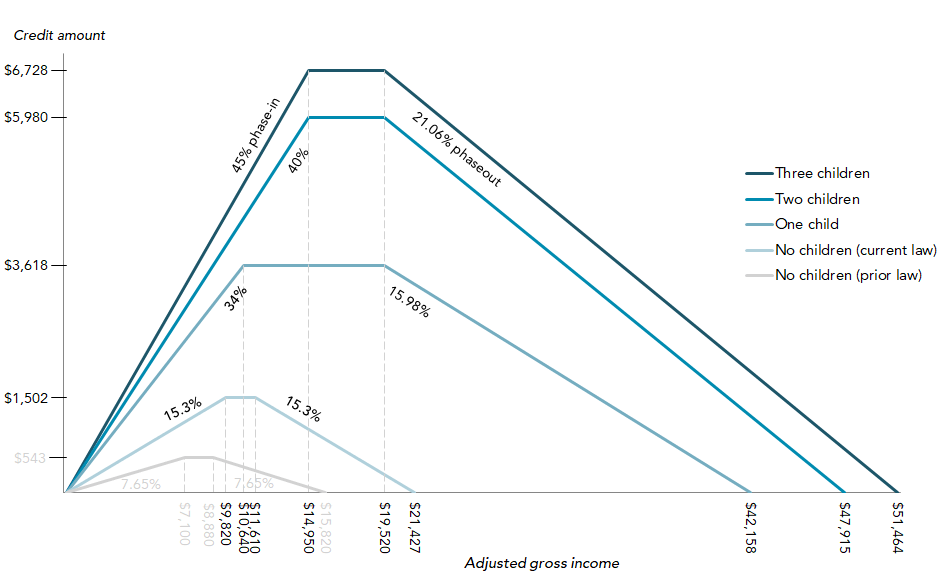
\includegraphics[width=.85\textwidth]{eitc_design}
    \end{center}
	\footnotesize
    \label{fig:tax}{Source: Tax Policy Center}
\end{figure}

Proponents of the EITC generally argue that it avoids the adverse incentives of other traditional welfare programs by encouraging workforce participation while simultaneously targeting low-income earners. Economic theory would suggest that the EITC would be especially pronounced at the point of entry for the labor supply, encouraging those on the sidelines to enter the workforce because it rewards earnings and gives no payout if the tax filer is not in the labor force \citep{eissa2006behavioral}. EITCs also avoid the mired debates about the minimum wage by increasing earnings for workers without shifting the cost to employers. In short, EITCs enjoy support from a diverse coalition of policymakers for the purpose of raising the earned income of low-wage individuals and families, without discouraging work.

Because of the dual-pronged motivation of the EITC, most economists have been interested in studying the effects on poverty and labor supply. While the causal effects of the federal program can be difficult to discern, \cite{neumark2001using} found that the EITC effectively raised a number of households above the poverty line and positively increased the labor supply rate, particularly at the point of labor entry, finding it to be a more effective intervention than the minimum wage. Given the trapezoidal shape of the policy, economic theory would also suggest that it creates natural “kink points” in the earned income of workers.  \cite{saez2010taxpayers} finds some evidence that workers bunch at the phase-out kink point, but very little evidence that workers choose to reduce hours during the phase-in period. Meanwhile, since the EITC does not provide any benefit to individuals who are not working, it should have a direct impact on labor force participation decisions at the extensive margin (the decision to enter the workforce), but others have argued that the effect at the margins is negligible \citep{kleven2019eitc}. There is also some evidence that the incentives are obfuscated by the complicated nature of tax law \citep{chetty2013teaching}.

While the EITC is available to single filers without children, the benefits afforded to those workers are relatively modest compared to the credit given to workers with dependents. Therefore, much of the literature has focused on the effects on low-income families, especially single mothers. \cite{ evans2014giving} found that indicators of health and self-reported well-being of single mothers both increased with the expansion of the federal credit in 1993. Other papers have explored the EITC’s effect on birth rates \citep{baughman2003did}.

In the wake of the federal EITC and its various expansions, more than 25 states have adopted their own state-level EITCs to supplement low-income earners at the local level. State-level EITC’s generally function as a proportion of the federal credit, with a few exceptions (for example, Washington state has flat dollar amounts depending on household size). Amounts of state EITC vary significantly, from 5\% of the federal EITC amount (Louisiana) to 45\% (Maryland). We focus on the state-level EITCs that are refundable, meaning that even if a filer has no tax liability, they still receive a credit, effectively making their net tax amount negative. While some states offer non-refundable EITCs (meaning they can use the credit only to reduce their tax burden), we concentrate on the EITCs which function as a proper government cash transfer. All told, 23 states and the District of Columbia currently offer a state-level refundable EITC, and an additional 6 currently offer a non-refundable EITC, as seen in Table~\ref{fig:eitc_states}.

 \begin{longtable}[h]{lcc}
\caption{States with EITC}\\
 \hline
\\[-1.8ex] 
 State & \% of Federal EITC & Refundable \\ [0.5ex] 
 \hline\hline \\[-1.8ex] 
California$^{1}$ & Max $46.9\%$ & Yes \\
\\[-1.8ex] 
 Colorado & $10\%$ & Yes \\ 
\\[-1.8ex] 
 Connecticut & $23\%$ & Yes \\ 
\\[-1.8ex] 
 Delaware & $4.5\%$ & Yes \\ 
\\[-1.8ex] 
 Hawaii & $20\%$  & No \\ 
\\[-1.8ex] 
 Illinois & $18\%$ & Yes \\
\\[-1.8ex] 
 Indiana & $9\%$ & Yes \\
\\[-1.8ex] 
 Iowa & $15\%$ & Yes \\
\\[-1.8ex] 
 Kansas & $17\%$ & Yes\\ 
\\[-1.8ex] 
 Louisiana & $5\%$ & Yes \\
\\[-1.8ex] 
 Maine & $12\%$ & Yes \\
\\[-1.8ex] 
 Maryland & $45\%$ & Yes\\ 
\\[-1.8ex] 
 Massachusetts & $30\%$ & Yes\\
\\[-1.8ex] 
 Michigan & $6\%$ & Yes \\
\\[-1.8ex] 
 Minnesota$^{2}$ & $25\%$ to $45\%$ & Yes  \\
\\[-1.8ex] 
 Montana & $3\%$ & Yes  \\
\\[-1.8ex] 
 Nebraska & $10\%$ & Yes  \\
\\[-1.8ex] 
 New Jersey & $40\%$ & Yes \\
\\[-1.8ex] 
 New Mexico & $20\%$ & Yes \\
\\[-1.8ex] 
 New York & $30\%$ & Yes \\
\\[-1.8ex] 
 Ohio & $30\%$ & No \\
\\[-1.8ex] 
 Oklahoma & $5\%$ & Yes \\
\\[-1.8ex] 
 Oregon & $9\%$ & Yes \\
\\[-1.8ex] 
 Rhode Island & $15\%$ & Yes \\
\\[-1.8ex] 
 South Carolina & $83.33\%$ & No \\
\\[-1.8ex] 
 Utah & $15\%$ & No \\
\\[-1.8ex] 
 Vermont & $36\%$ & Yes \\
\\[-1.8ex] 
 Virginia & $20\%$ & No \\
\\[-1.8ex] 
 Wisconsin$^{2}$ & $4\%$ to $34\%$ & Yes \\
\\[-1.8ex] 
 District of Columbia & $55\%$ & Yes \\
 \hline\\[-1.8ex] 
\footnotesize $^{1}$Uses different income thresholds than federal EITC\\
\footnotesize $^{2}$Percent changes by the number of children or income
\label{fig:eitc_states}{}
\end{longtable}



While there is substantial research on the federal Earned Income Tax Credit, literature on the state-level EITCs is much sparser. \cite{baughman2012effects} found some evidence that state EITCs improved child health in those states. Others have looked at the relationship between state EITCs and suicide \citep{lenhart2019effects} and how to increase uptake of state-level EITC credits \citep{linos2020can}. We therefore endeavor to apply the changes in EITC in California and North Carolina. 

In 2014, North Carolina eliminated its state-level EITC, the only state to do so in over 30 years. The eliminated benefit was modest, at 5\% of the federal EITC, but at the time of elimination, it was claimed by 22 percent of North Carolina residents. Conversely, in 2015, California created and implemented its first state EITC (CalEITC). This policy uses thresholds independent of the federal EITC, with CalEITC credits available up to \$3,160 for a family with three children (nearly half of the available federal EITC credit at that level). The Public Policy Institute of California estimates that in the first year of creation, the CalEITC was claimed by 14\% of households in the state, with more than 90\% of claimants having dependent children. They also estimate that without both state and federal EITCs, 840,000 more Californians would be in poverty, including an estimated 376,000 children.  


\section{Data}


\section{Methodology}


\section{Results}

In Figure~\ref{fig:series}, we compare how our synthetic California and North Carolina compare to their real counterparts in both labor force participation rate and poverty rate. Following the implementation of CalEITC in 2015, we see an increase in labor force participation (about half a percent) and a decrease poverty rate (about 1\%), relative to our synthetic California. We also see a similar decrease in labor force participation following the elimination of North Carolina's EITC. However, the poverty rate in North Carolina is also below the synthetic level, bucking the economic theory. Figure~\ref{fig:weights} shows how the weights of our synthetic controls are generated. 

\newgeometry{margin=.5in}

\begin{figure}
\begin{center}
\caption{Poverty and Labor Supply in California and North Carolina with Synthetic Control}
\begin{tabular}{cc}
 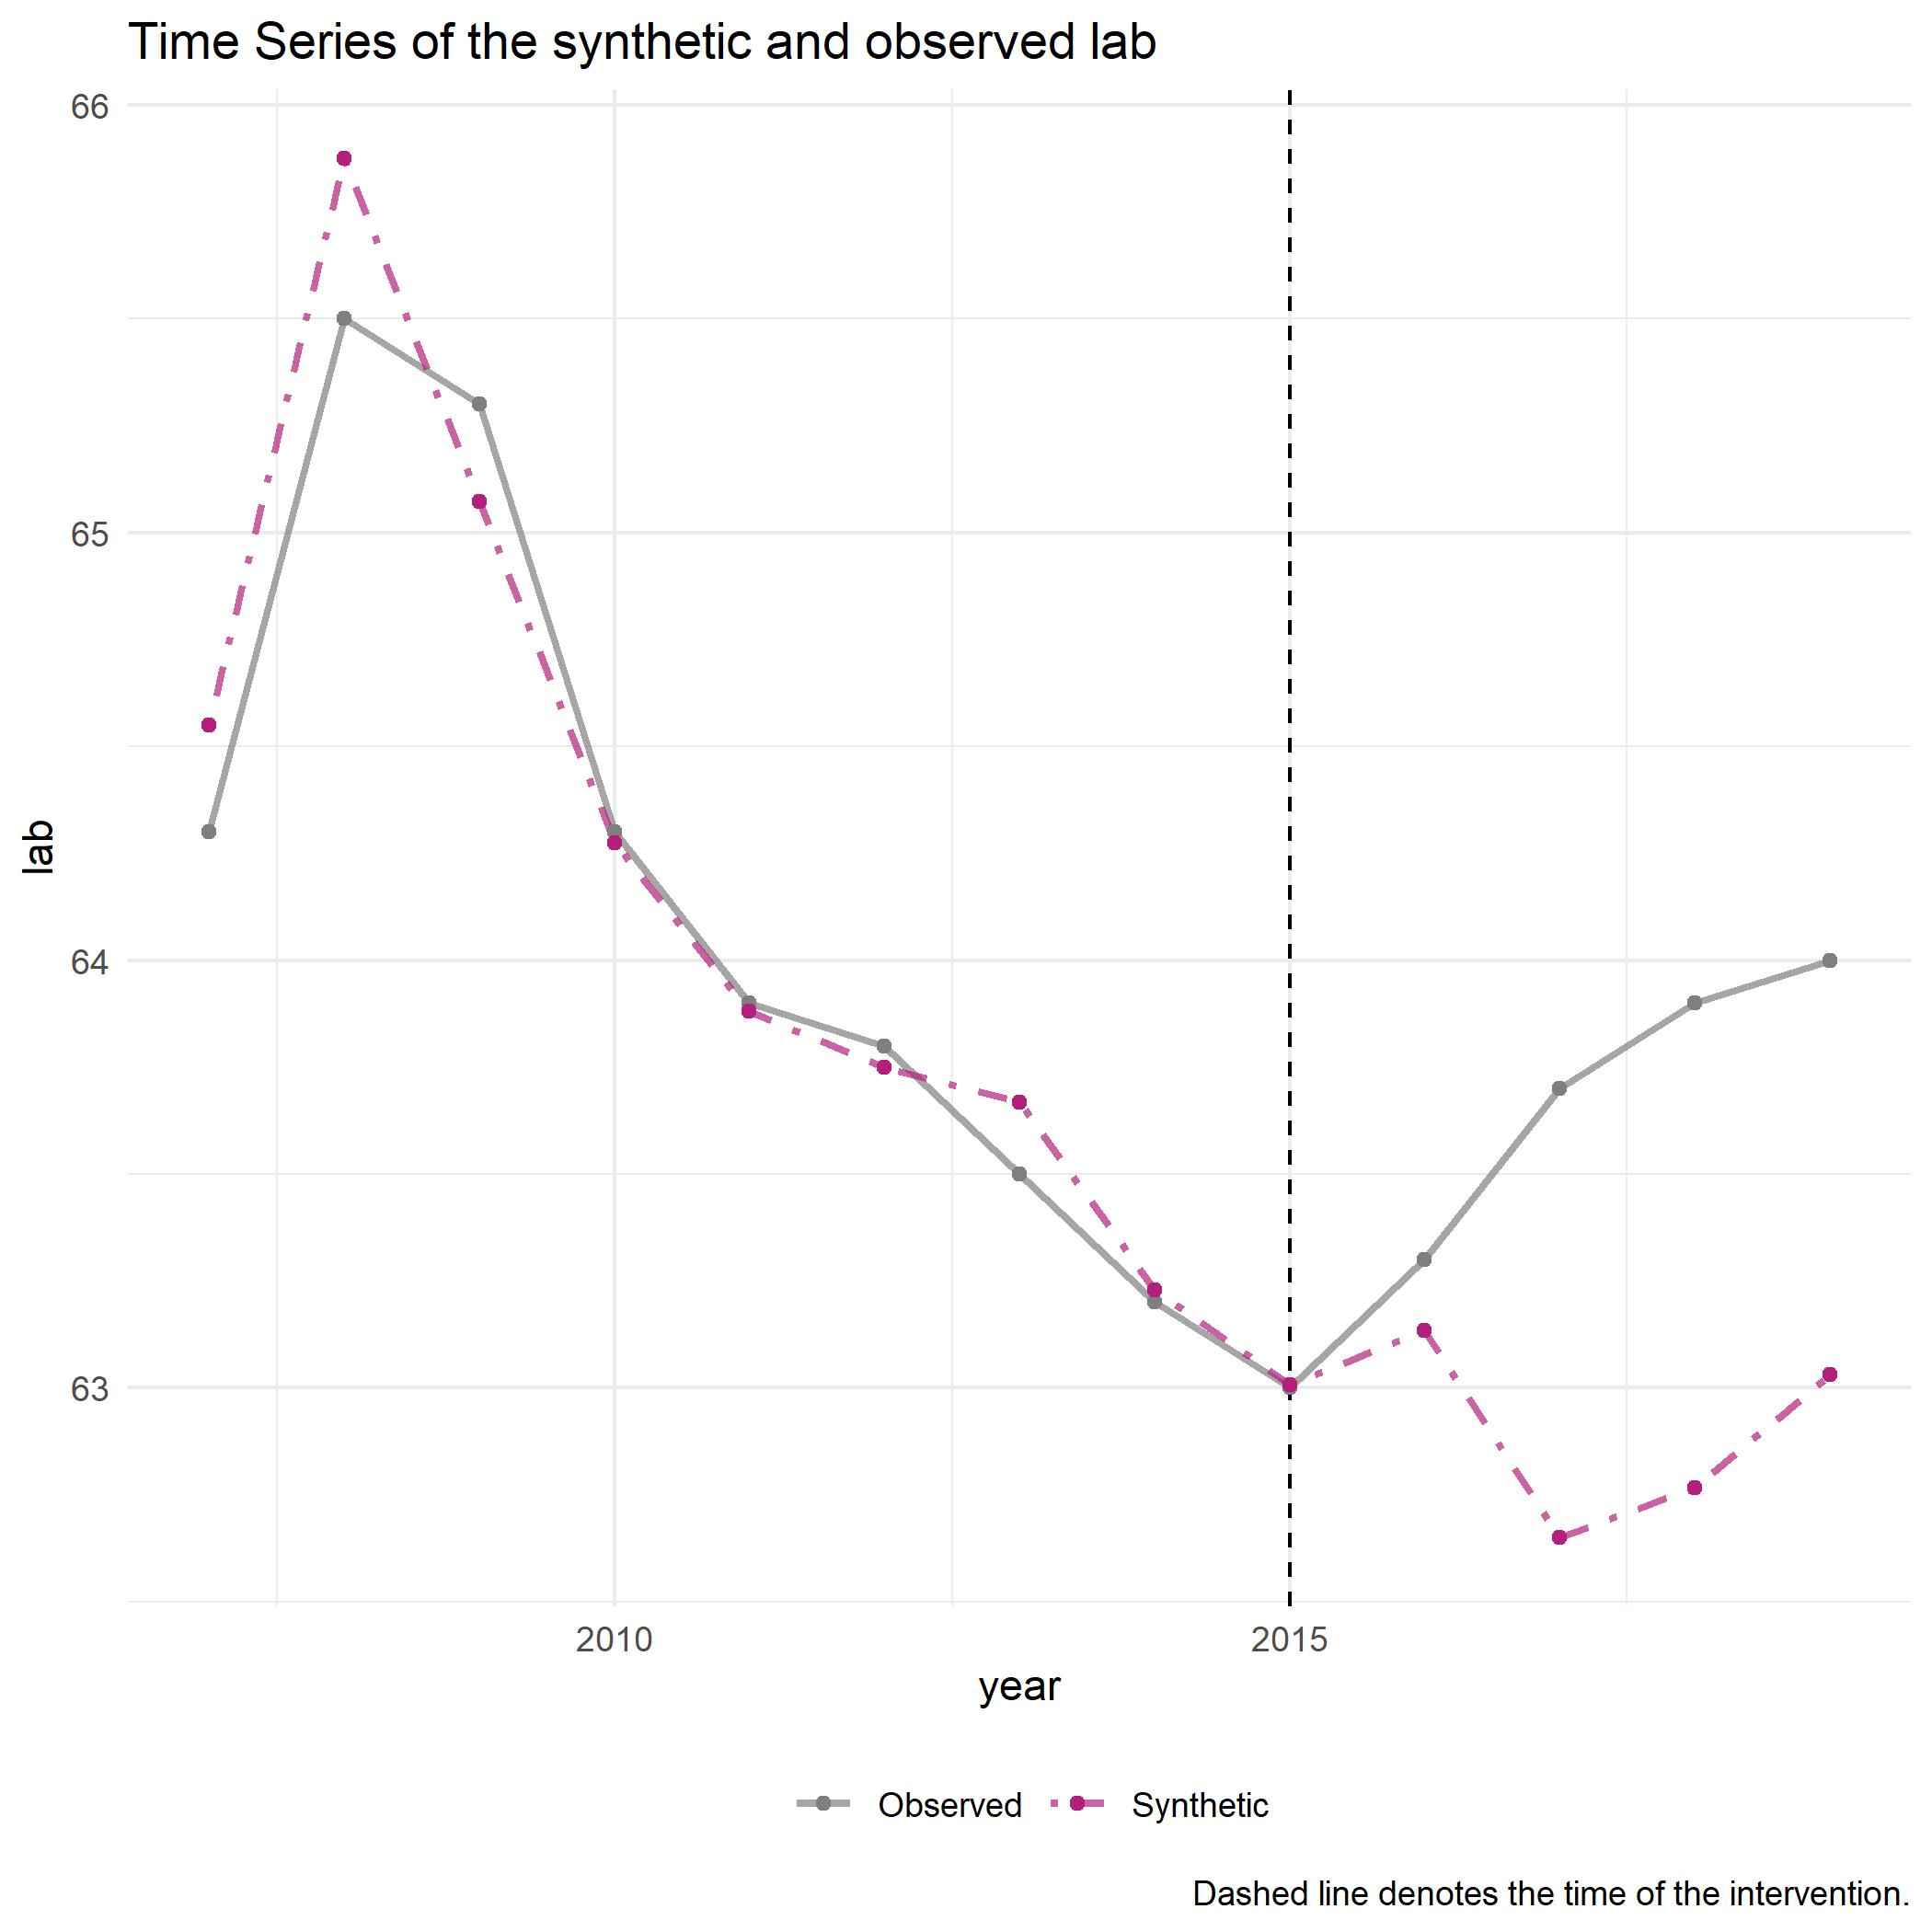
\includegraphics[width=80mm]{ca_lab_trend} &   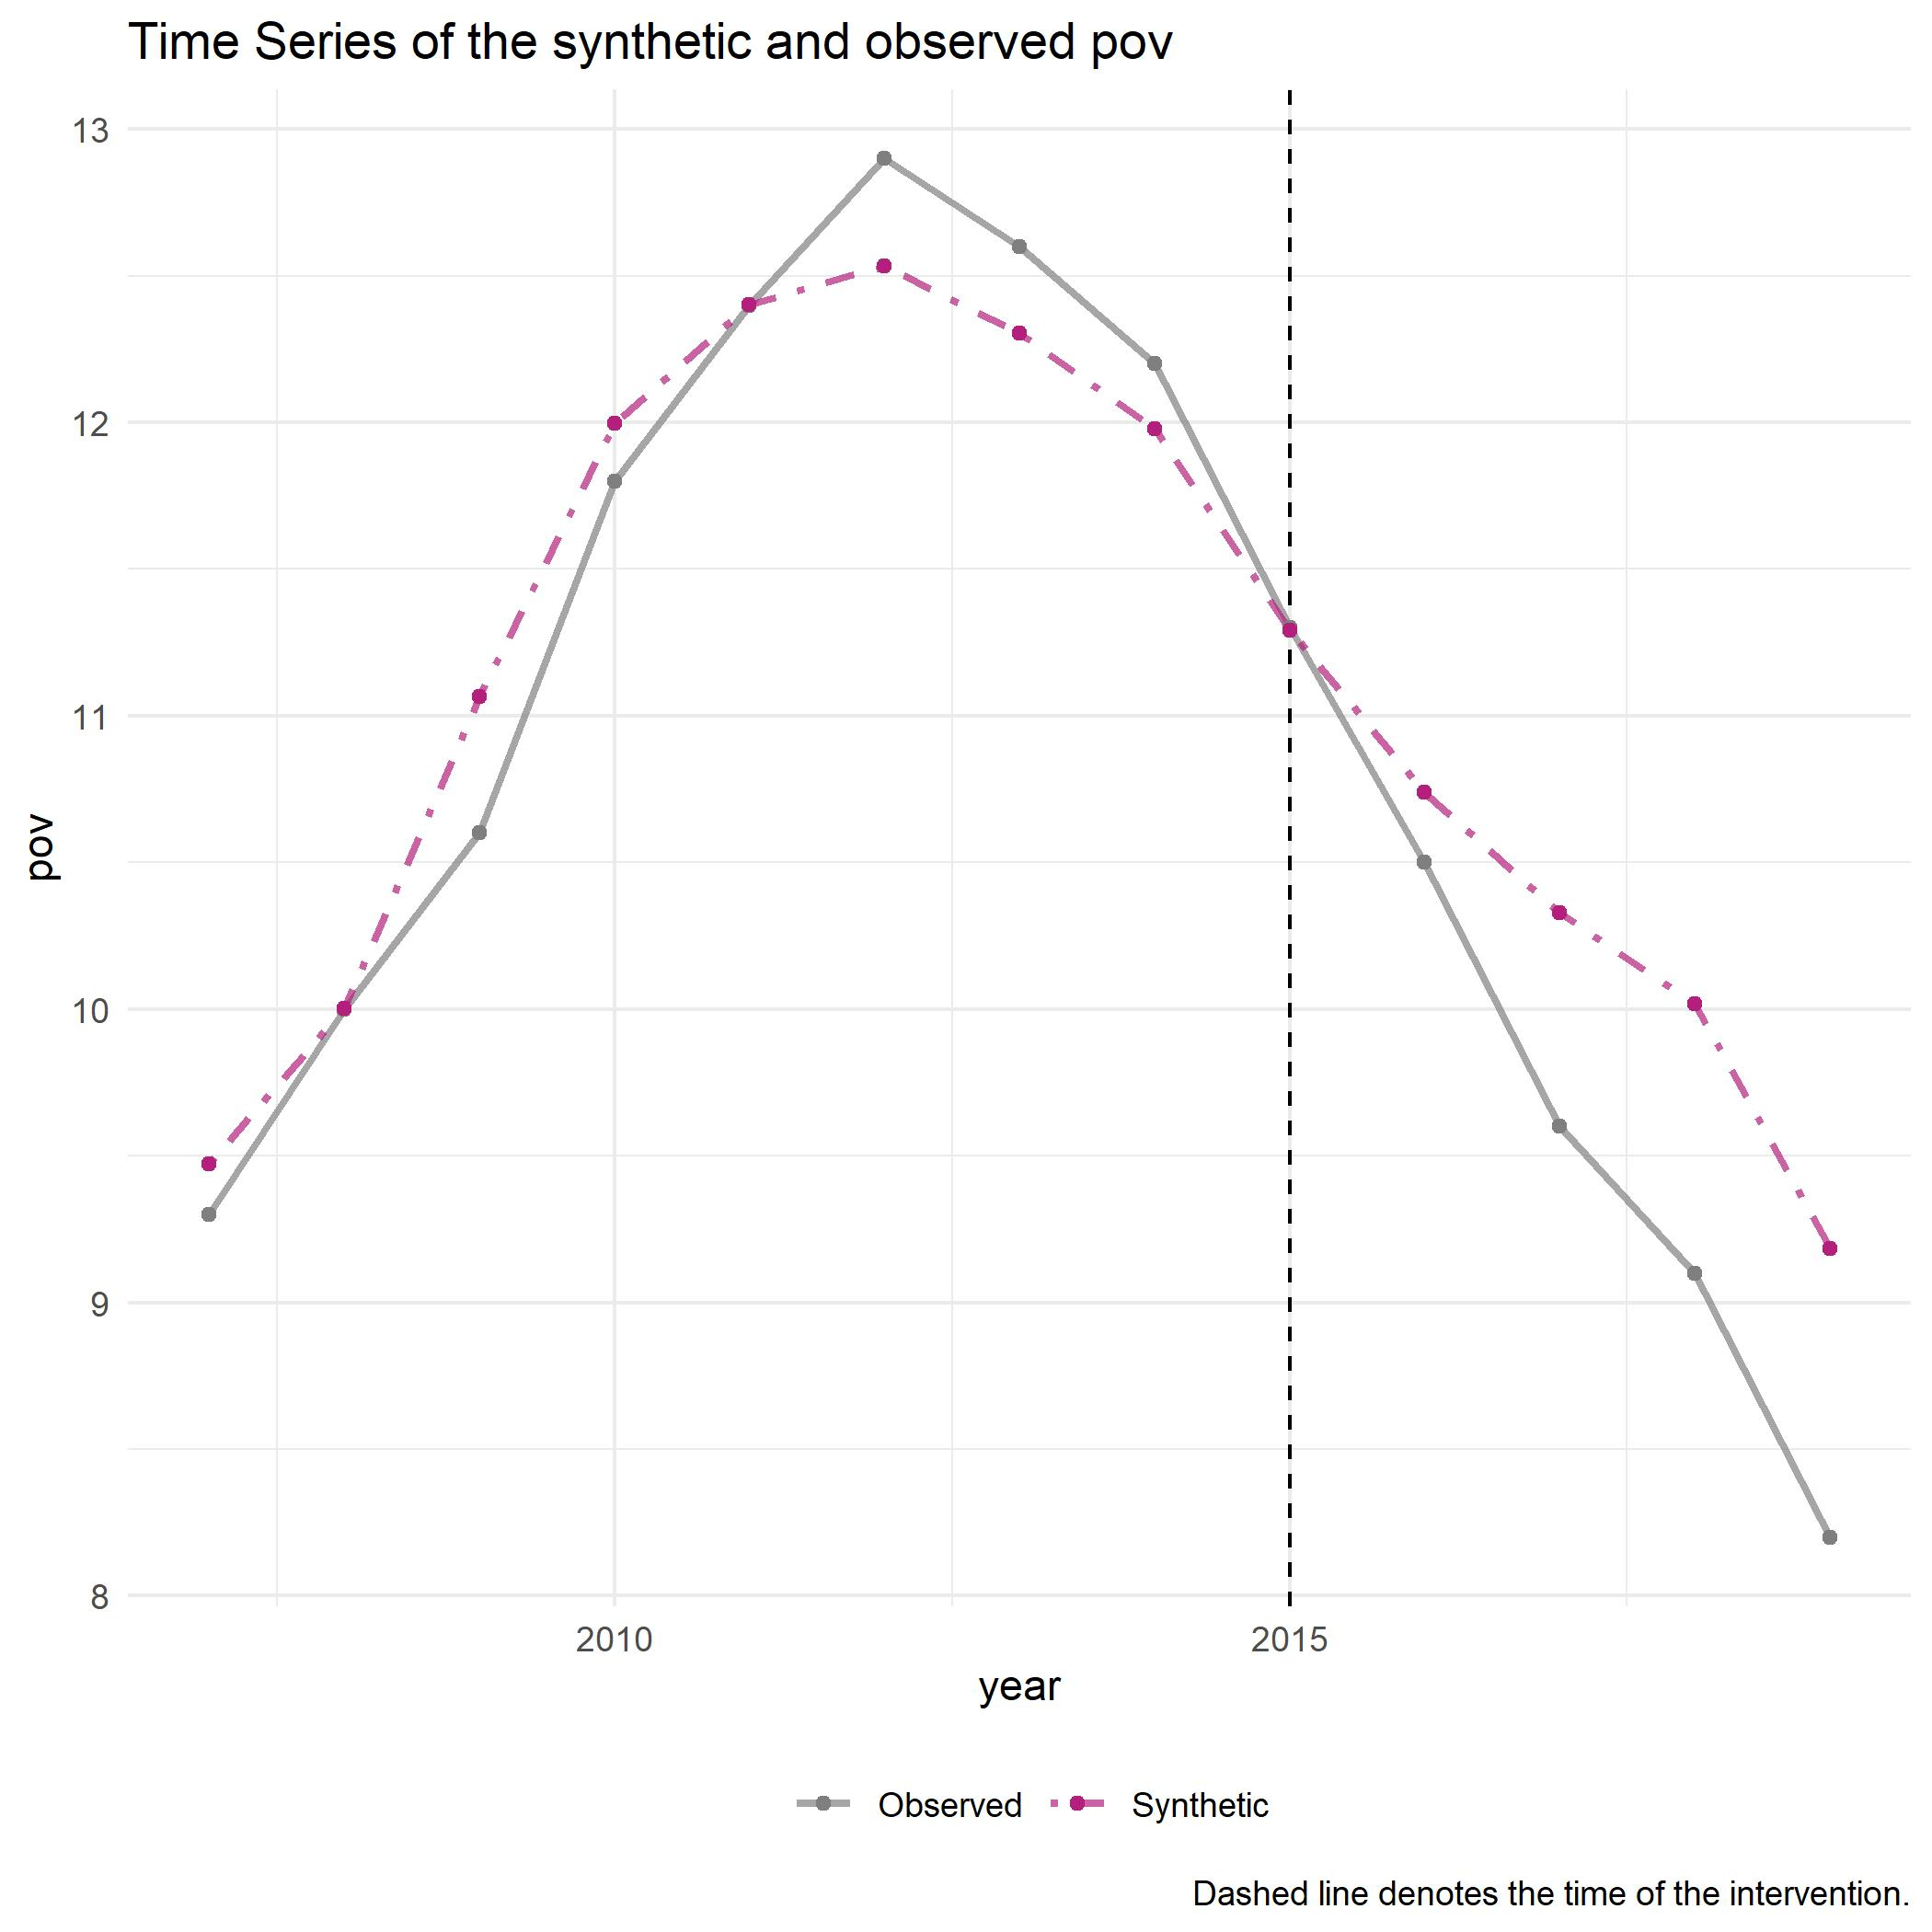
\includegraphics[width=80mm]{ca_pov_trend} \\
 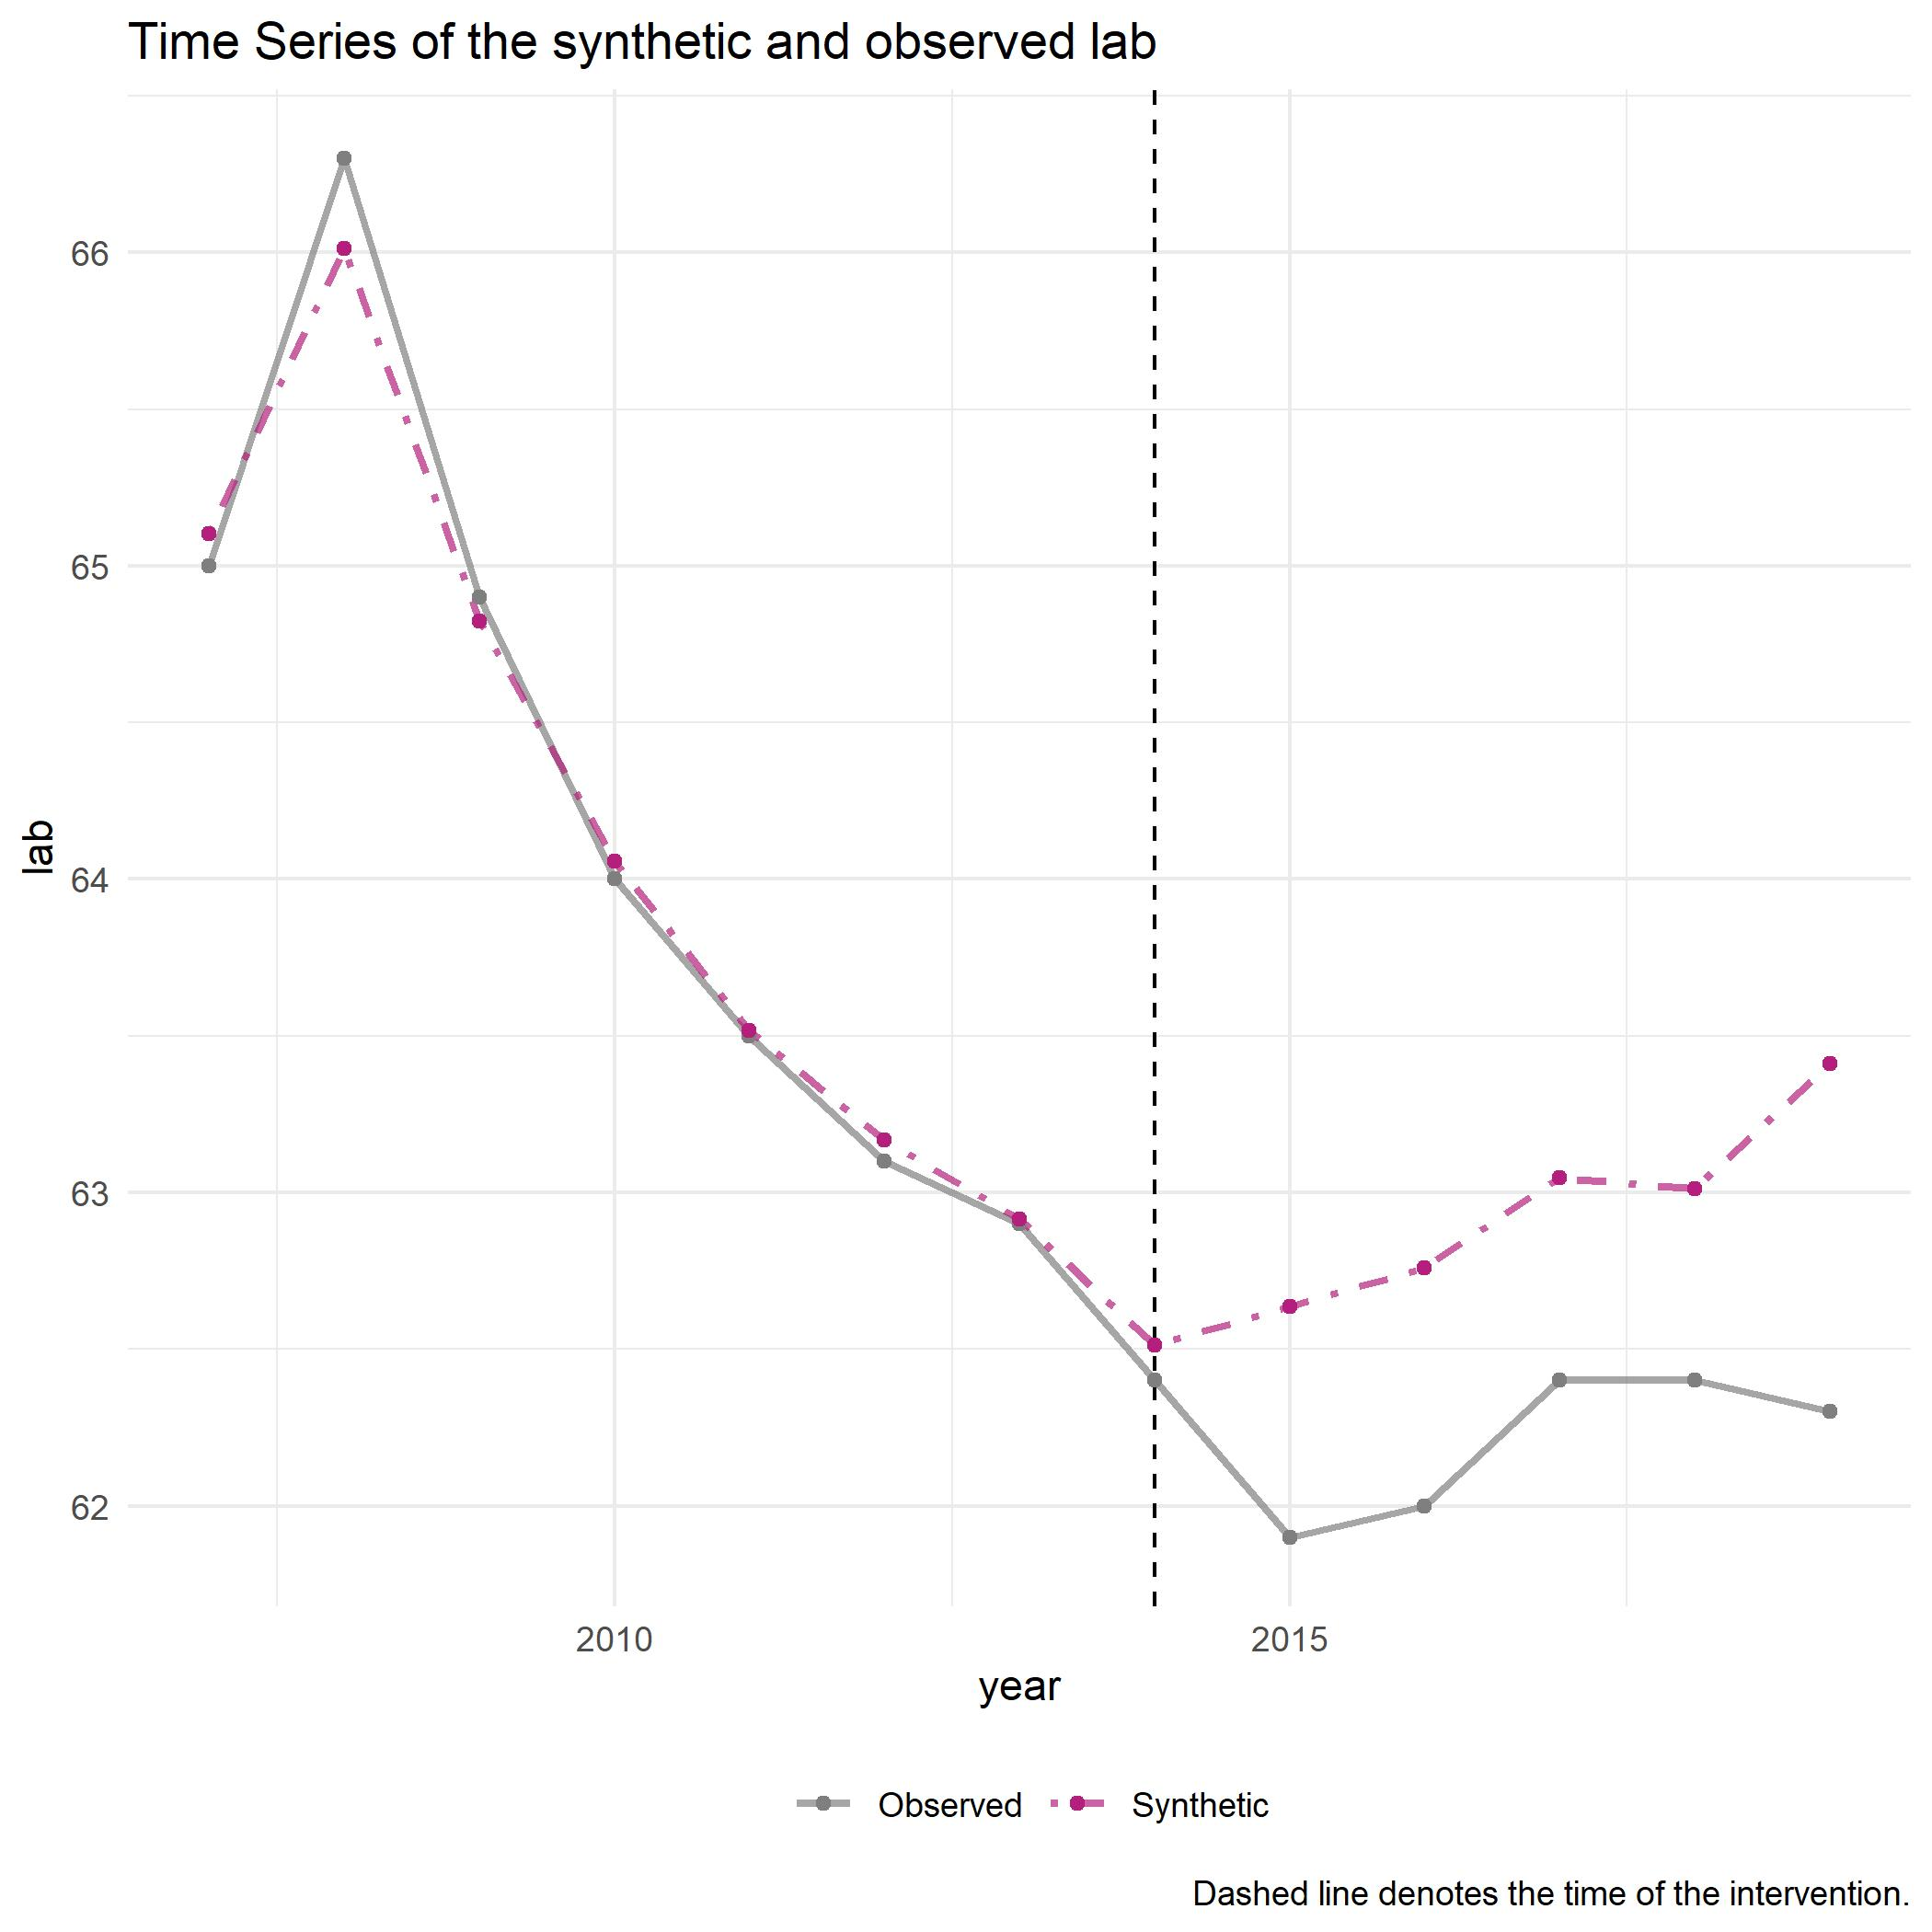
\includegraphics[width=80mm]{nc_lab_trend} &   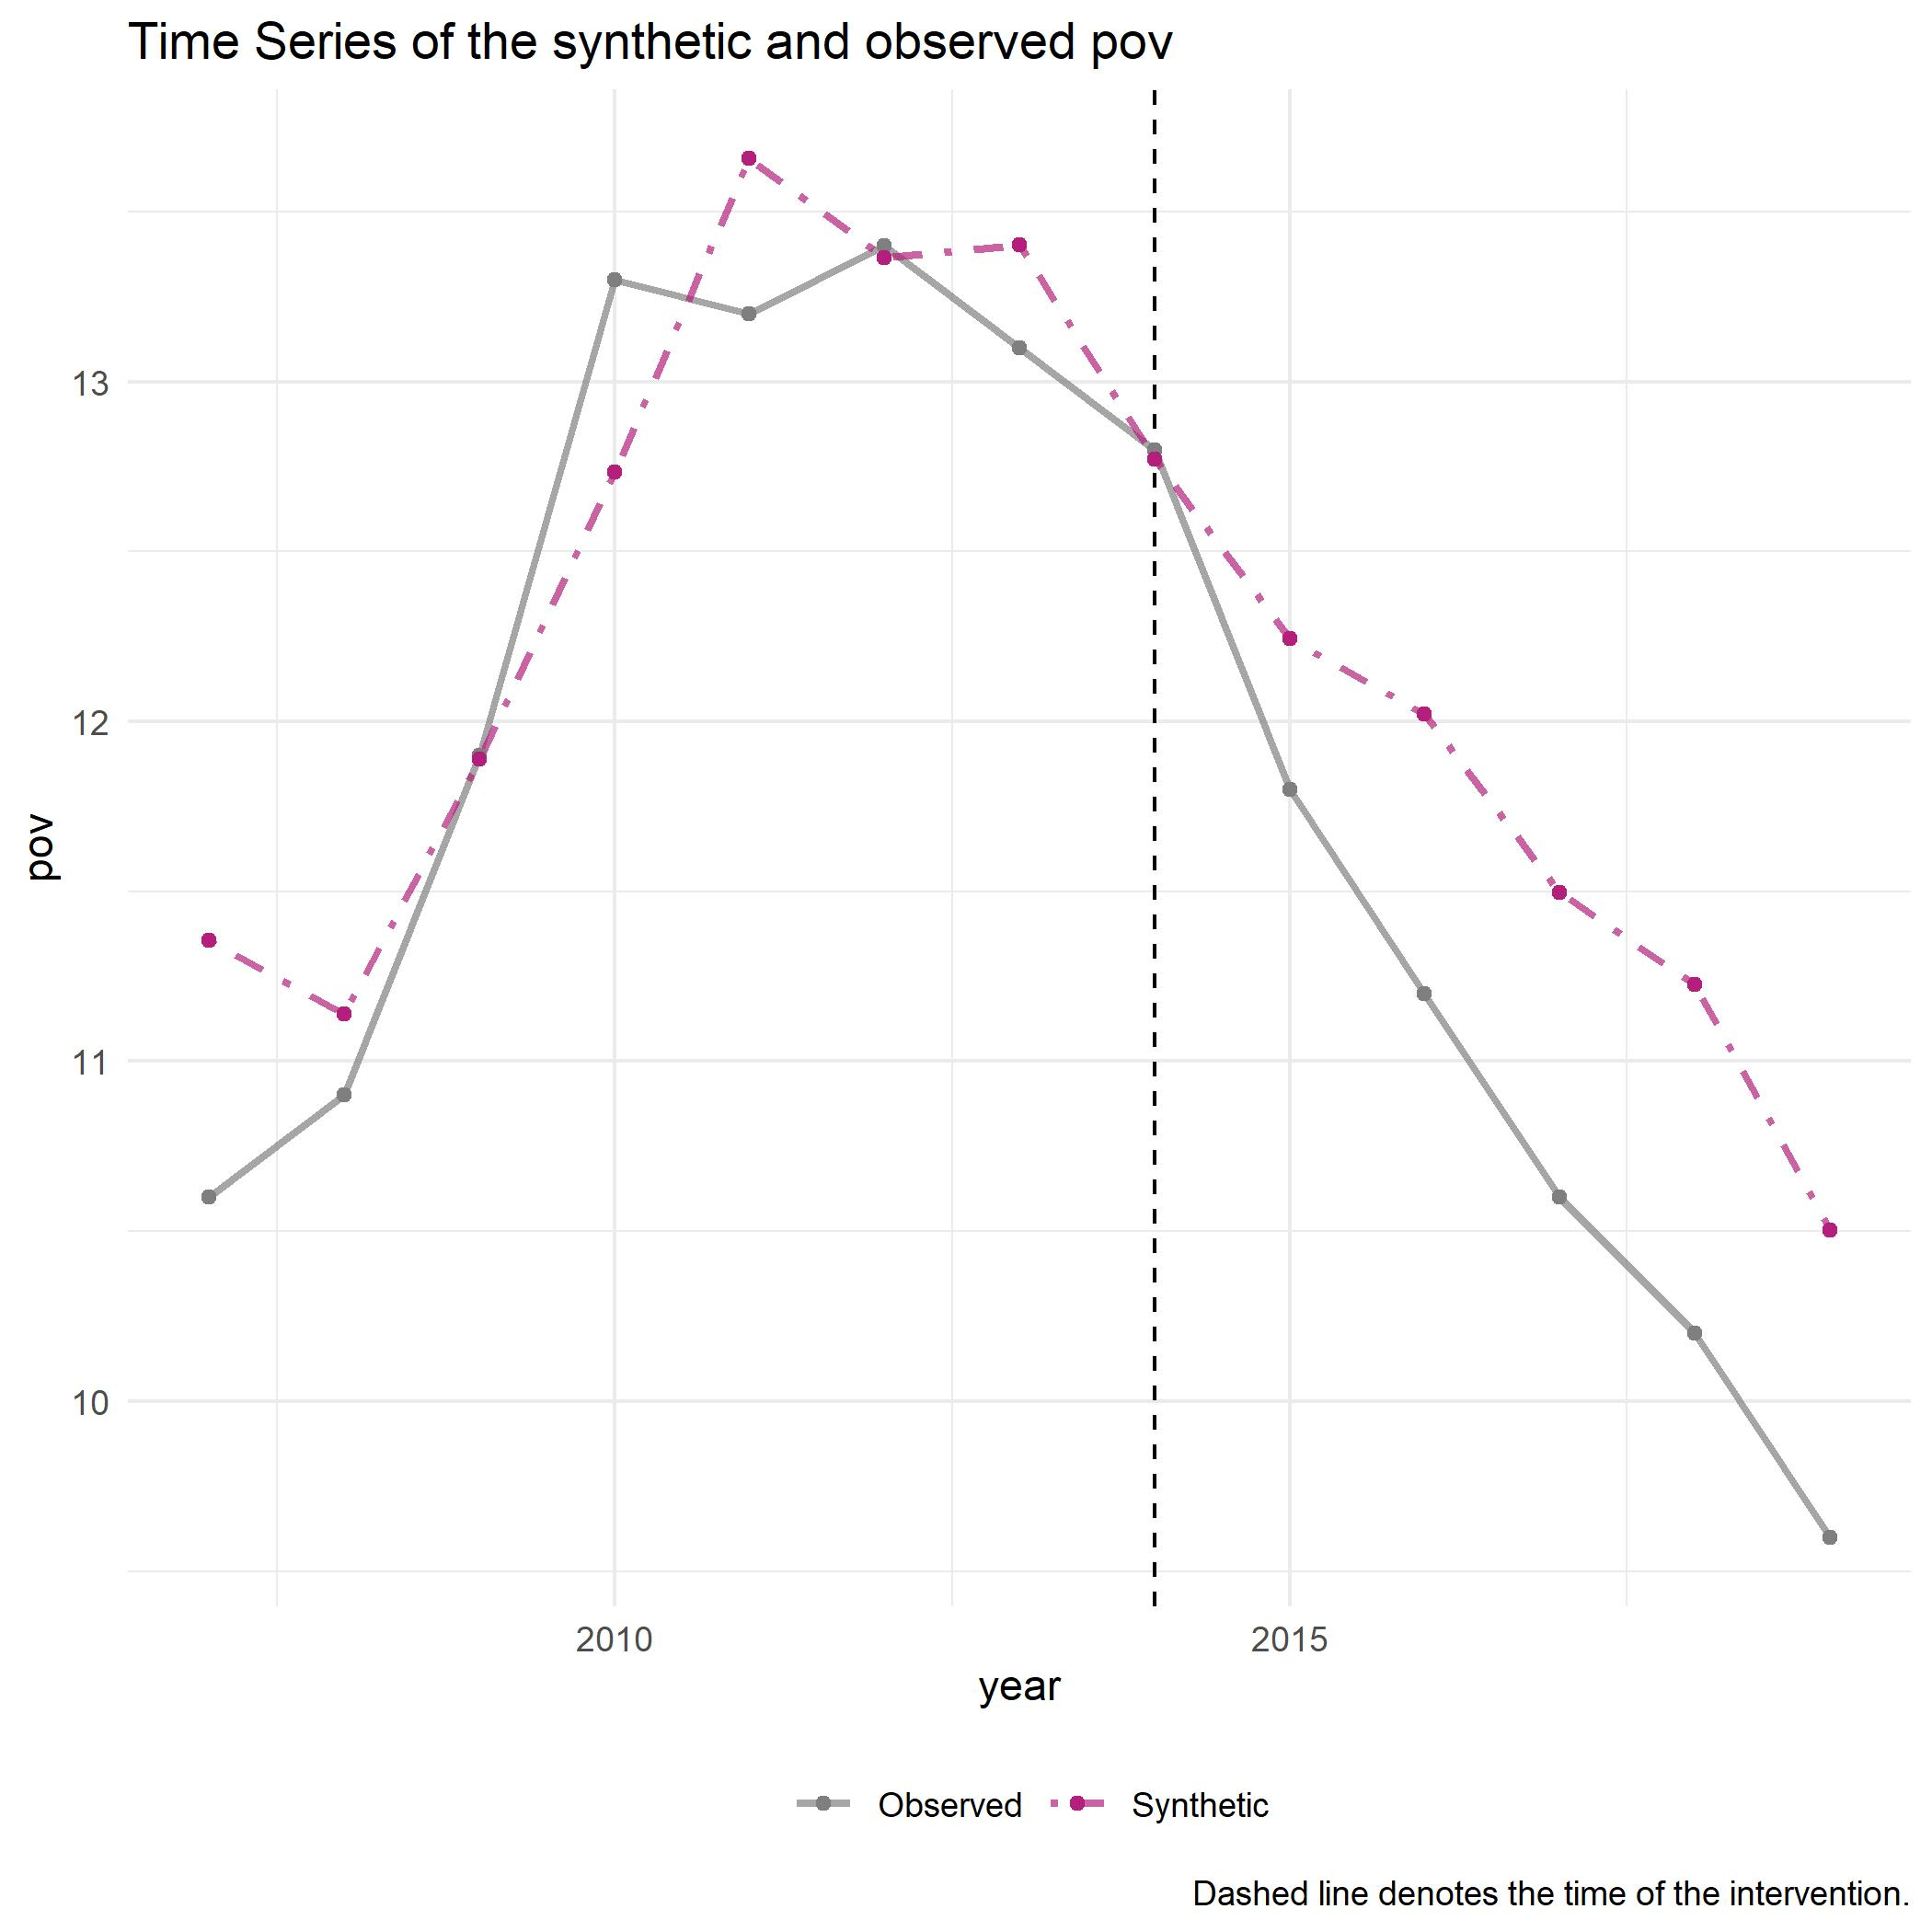
\includegraphics[width=80mm]{nc_pov_trend} \\
\end{tabular}
\end{center}
\label{fig:series}{}
\end{figure}

\restoregeometry

\newgeometry{margin=.5in}

\begin{figure}
\begin{center}
\caption{Weights Assigned for Synthetic California and North Carolina}
\begin{tabular}{cc}
 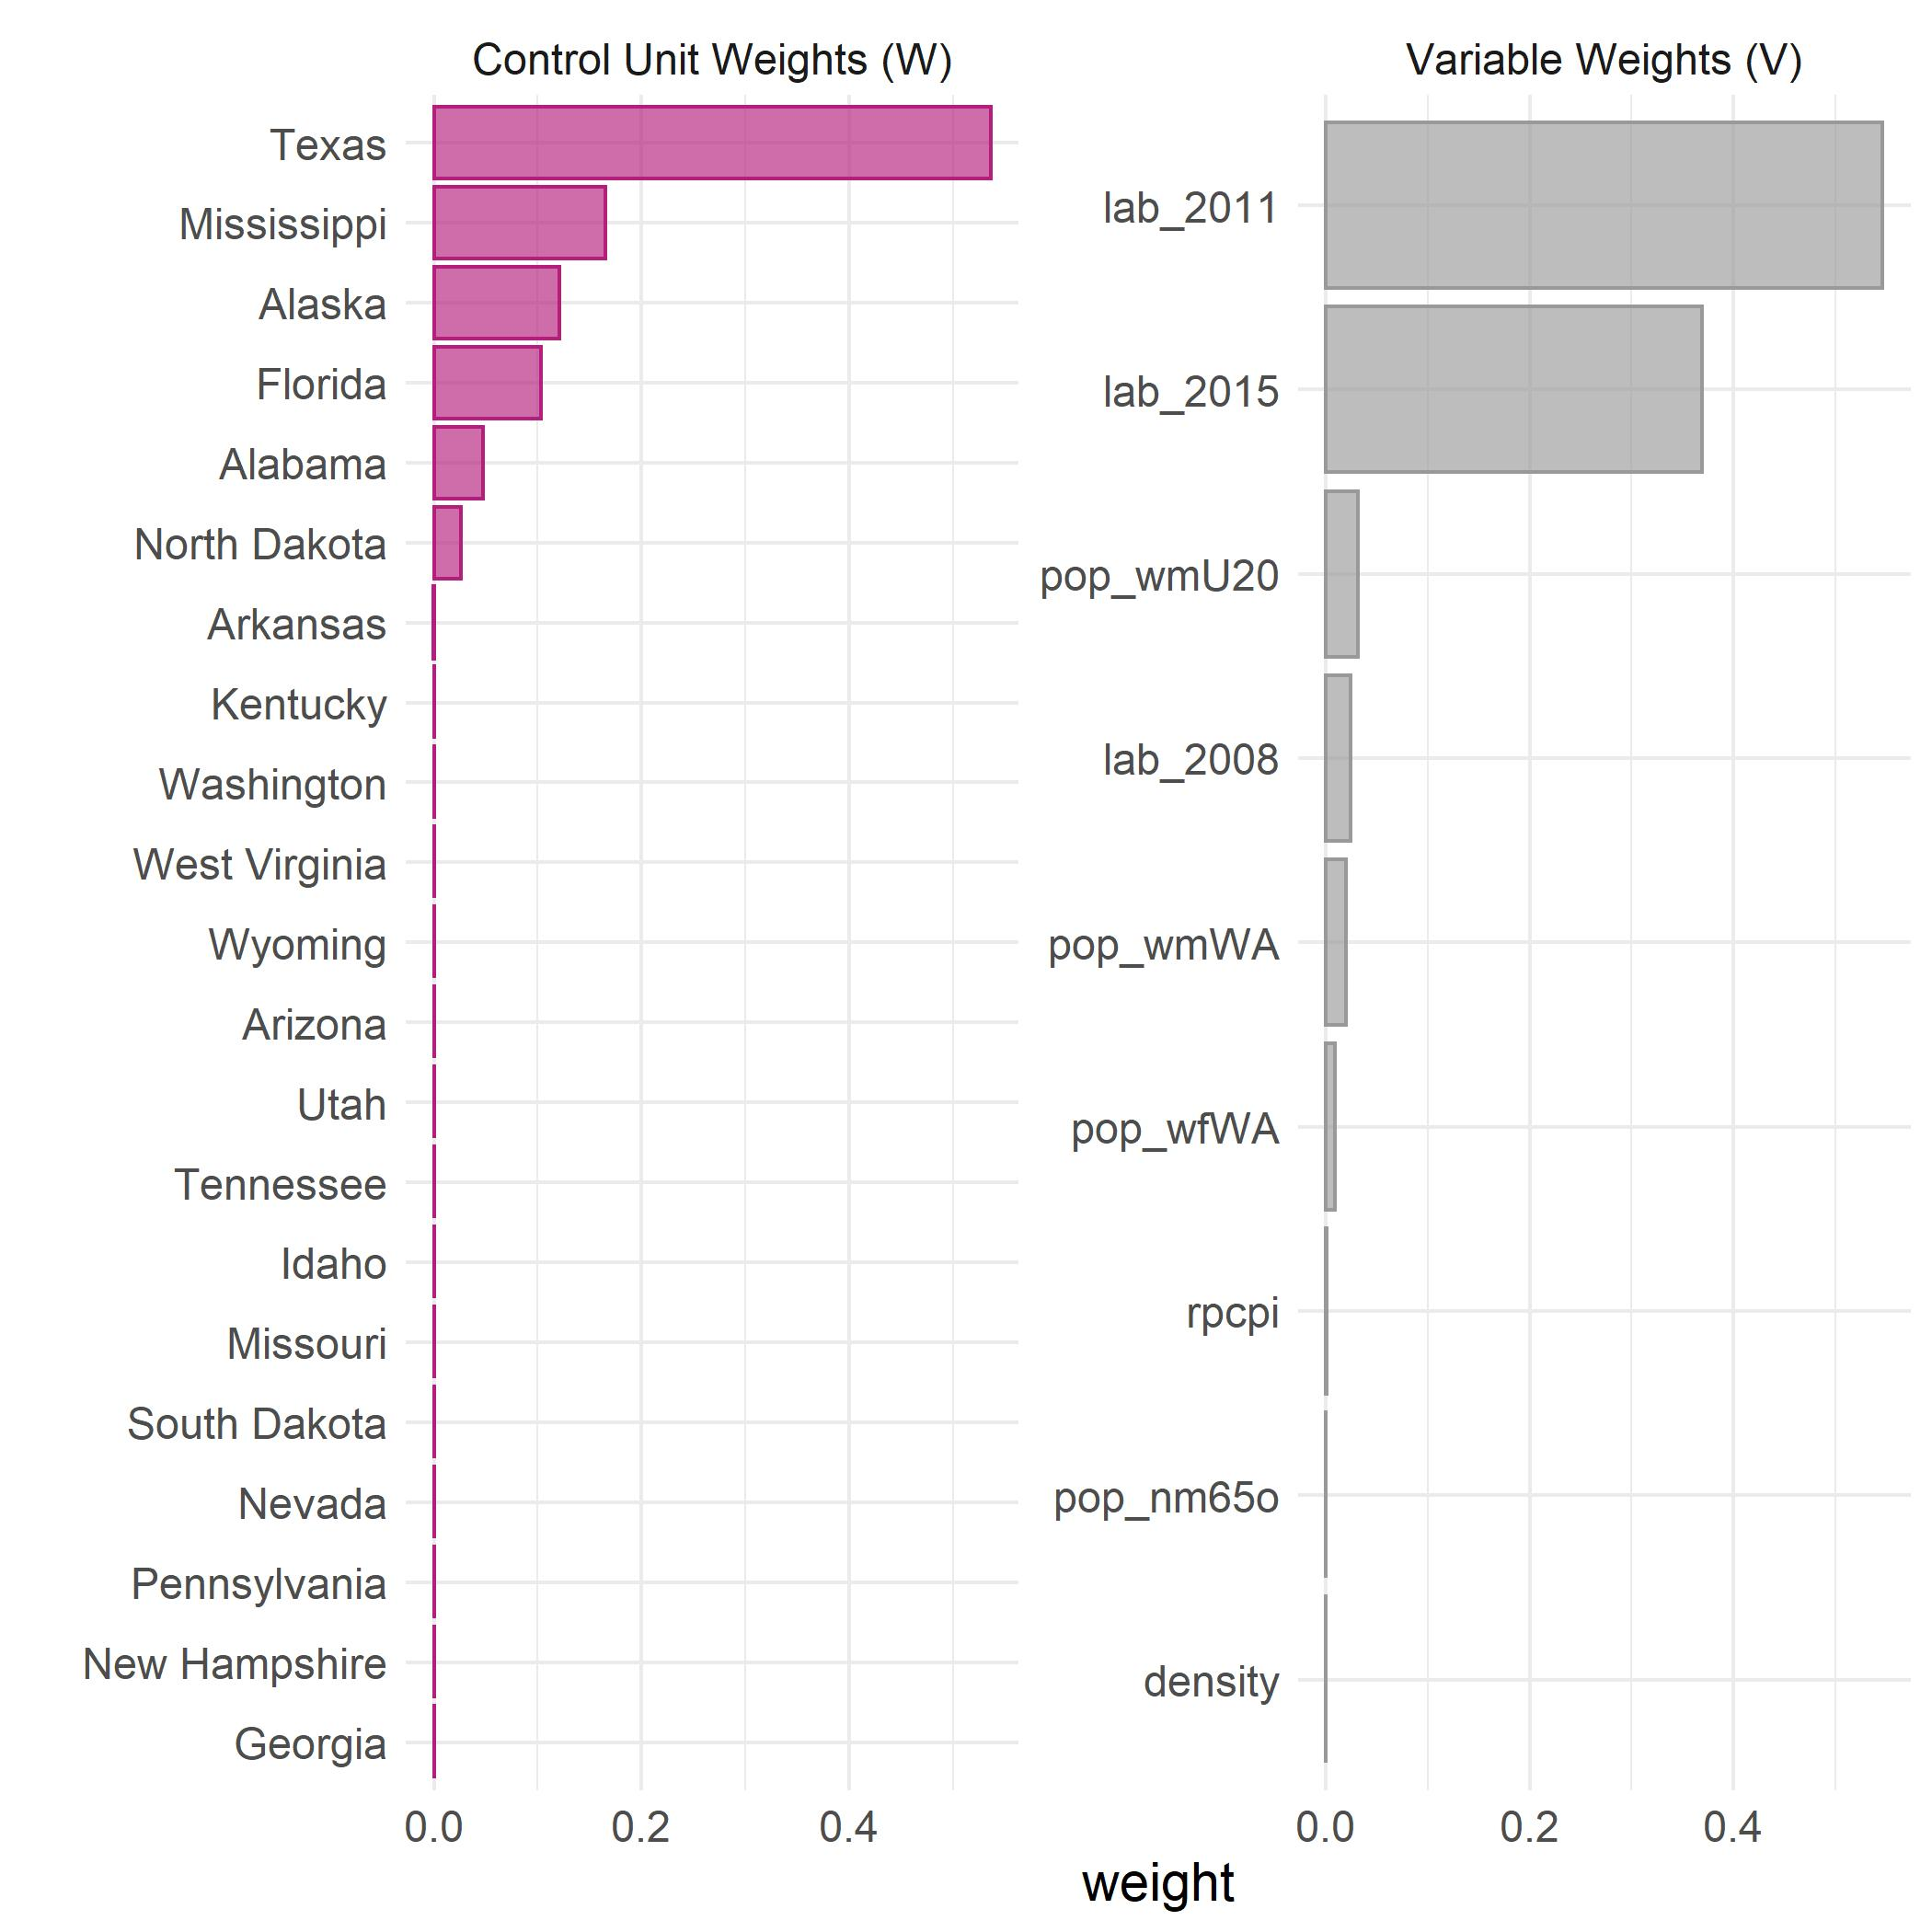
\includegraphics[width=80mm]{ca_lab_weights} &   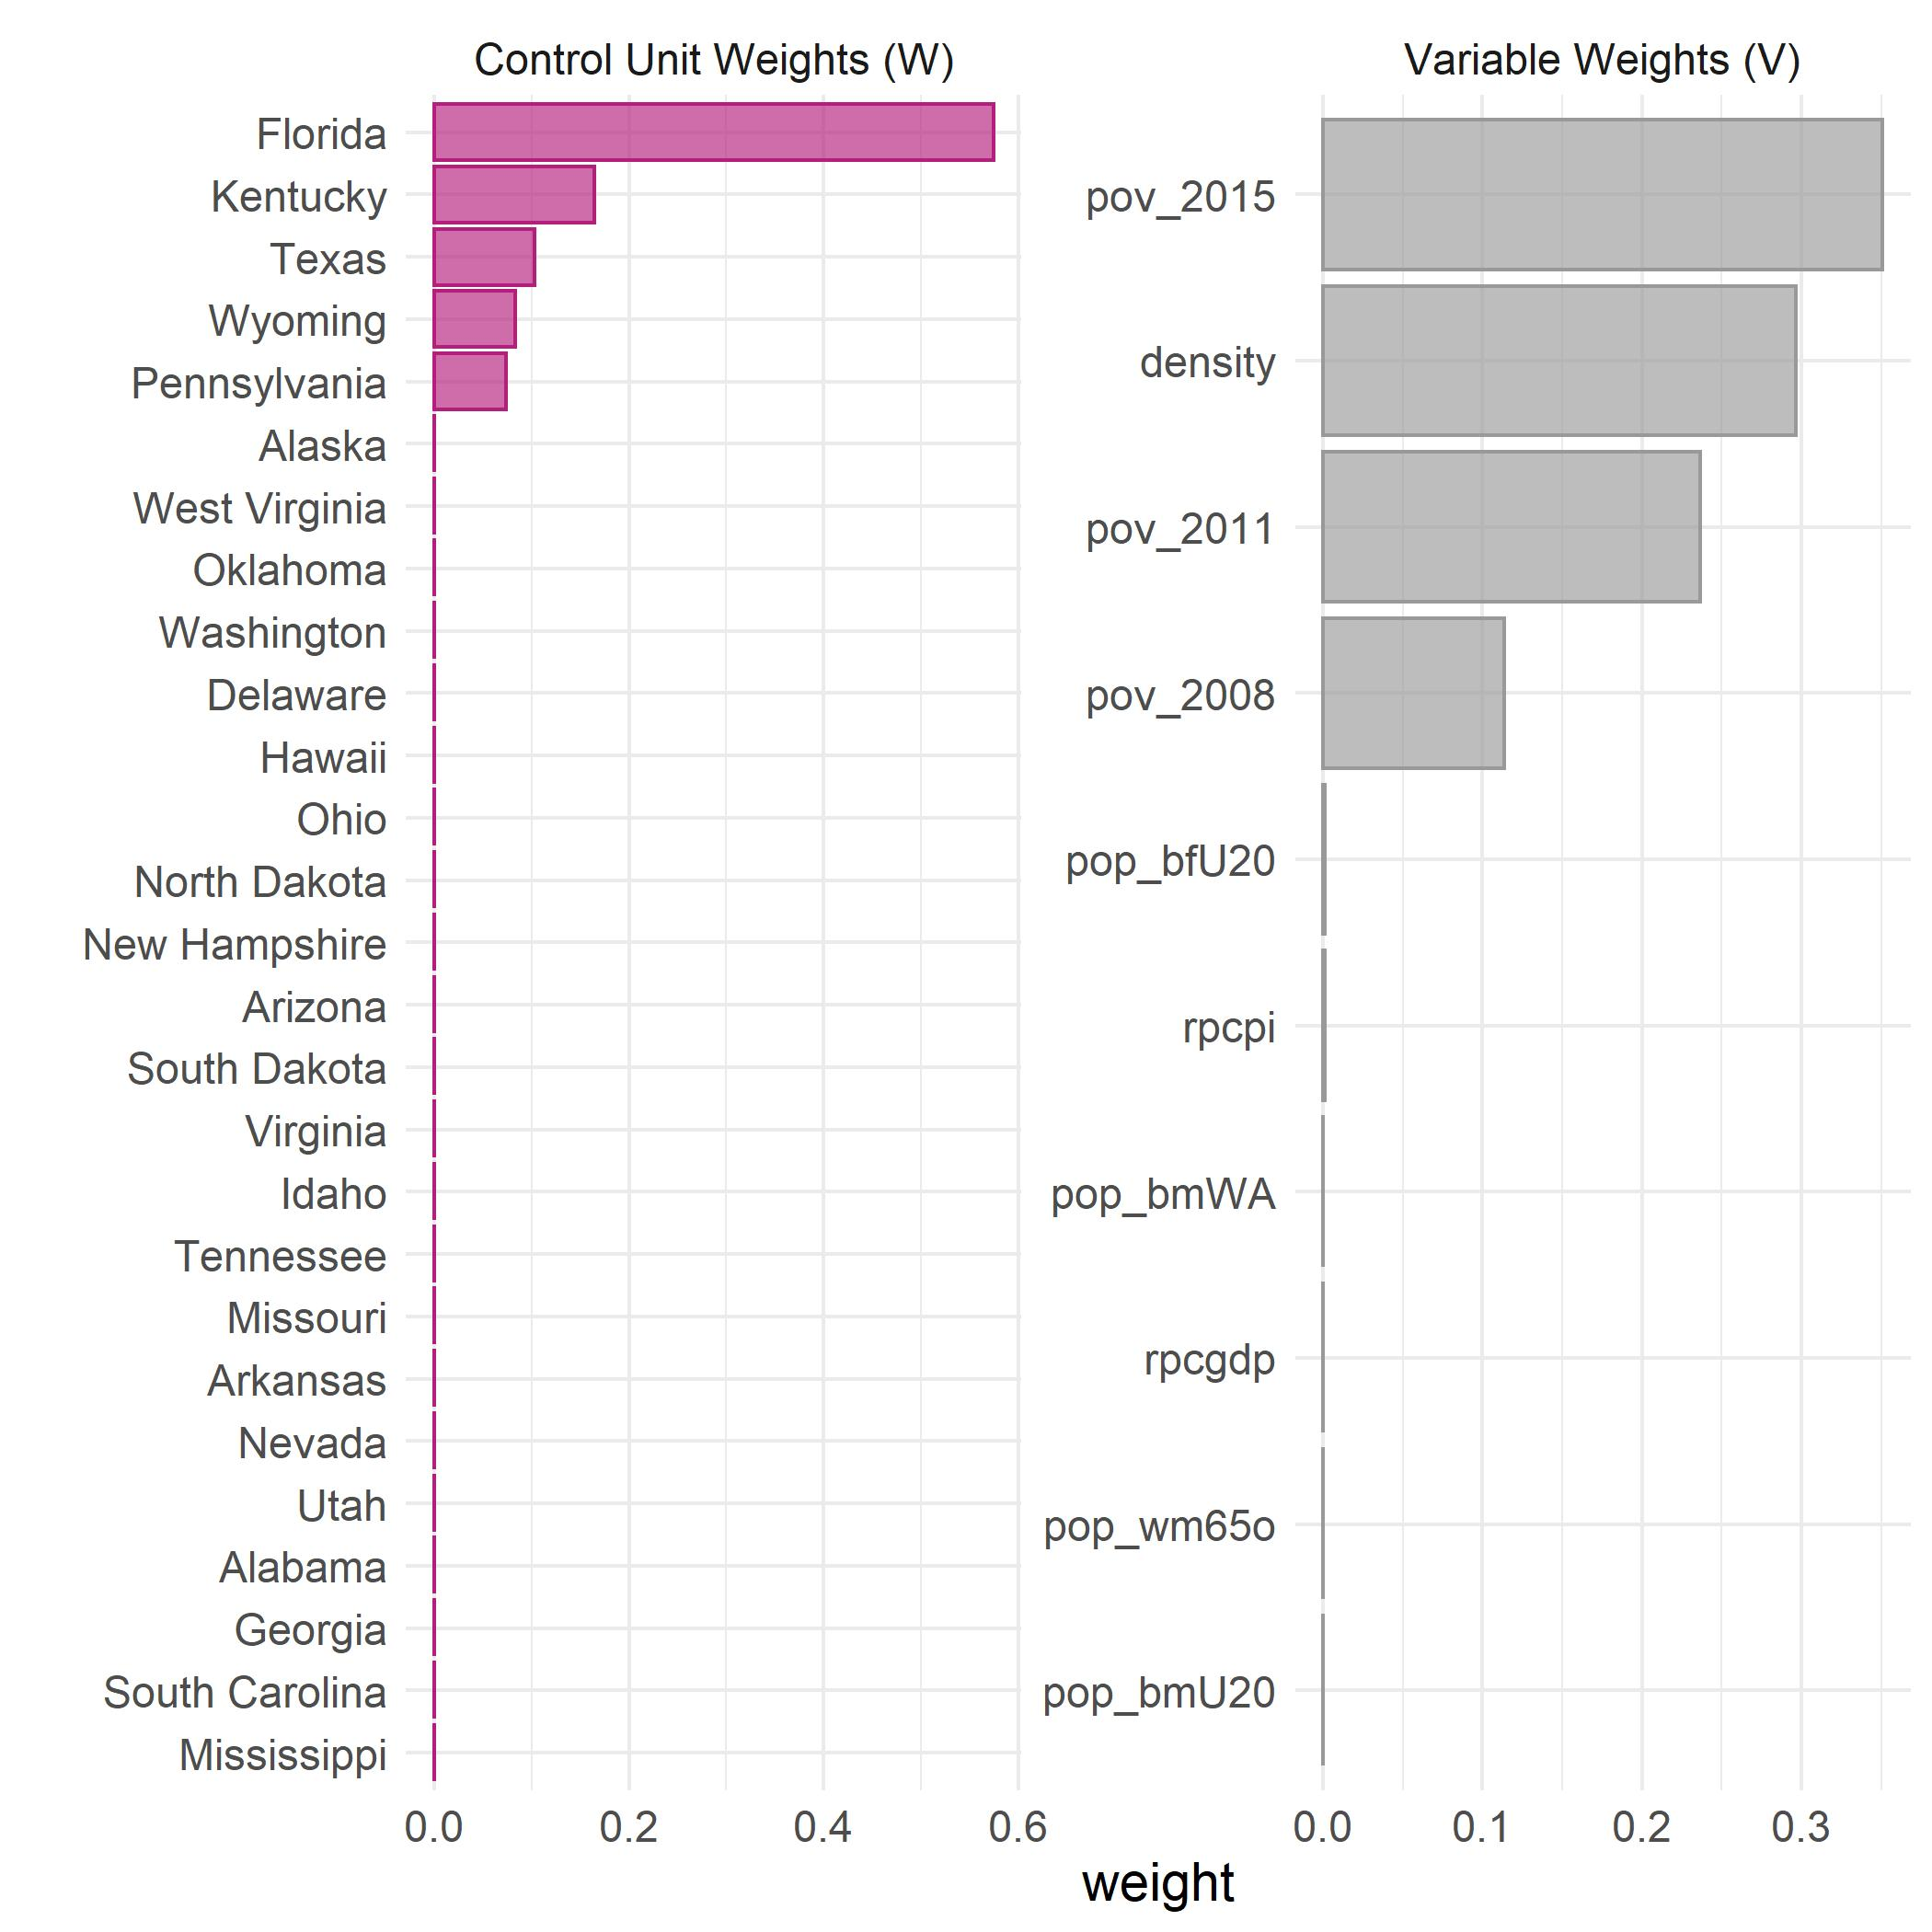
\includegraphics[width=80mm]{ca_pov_weights} \\
 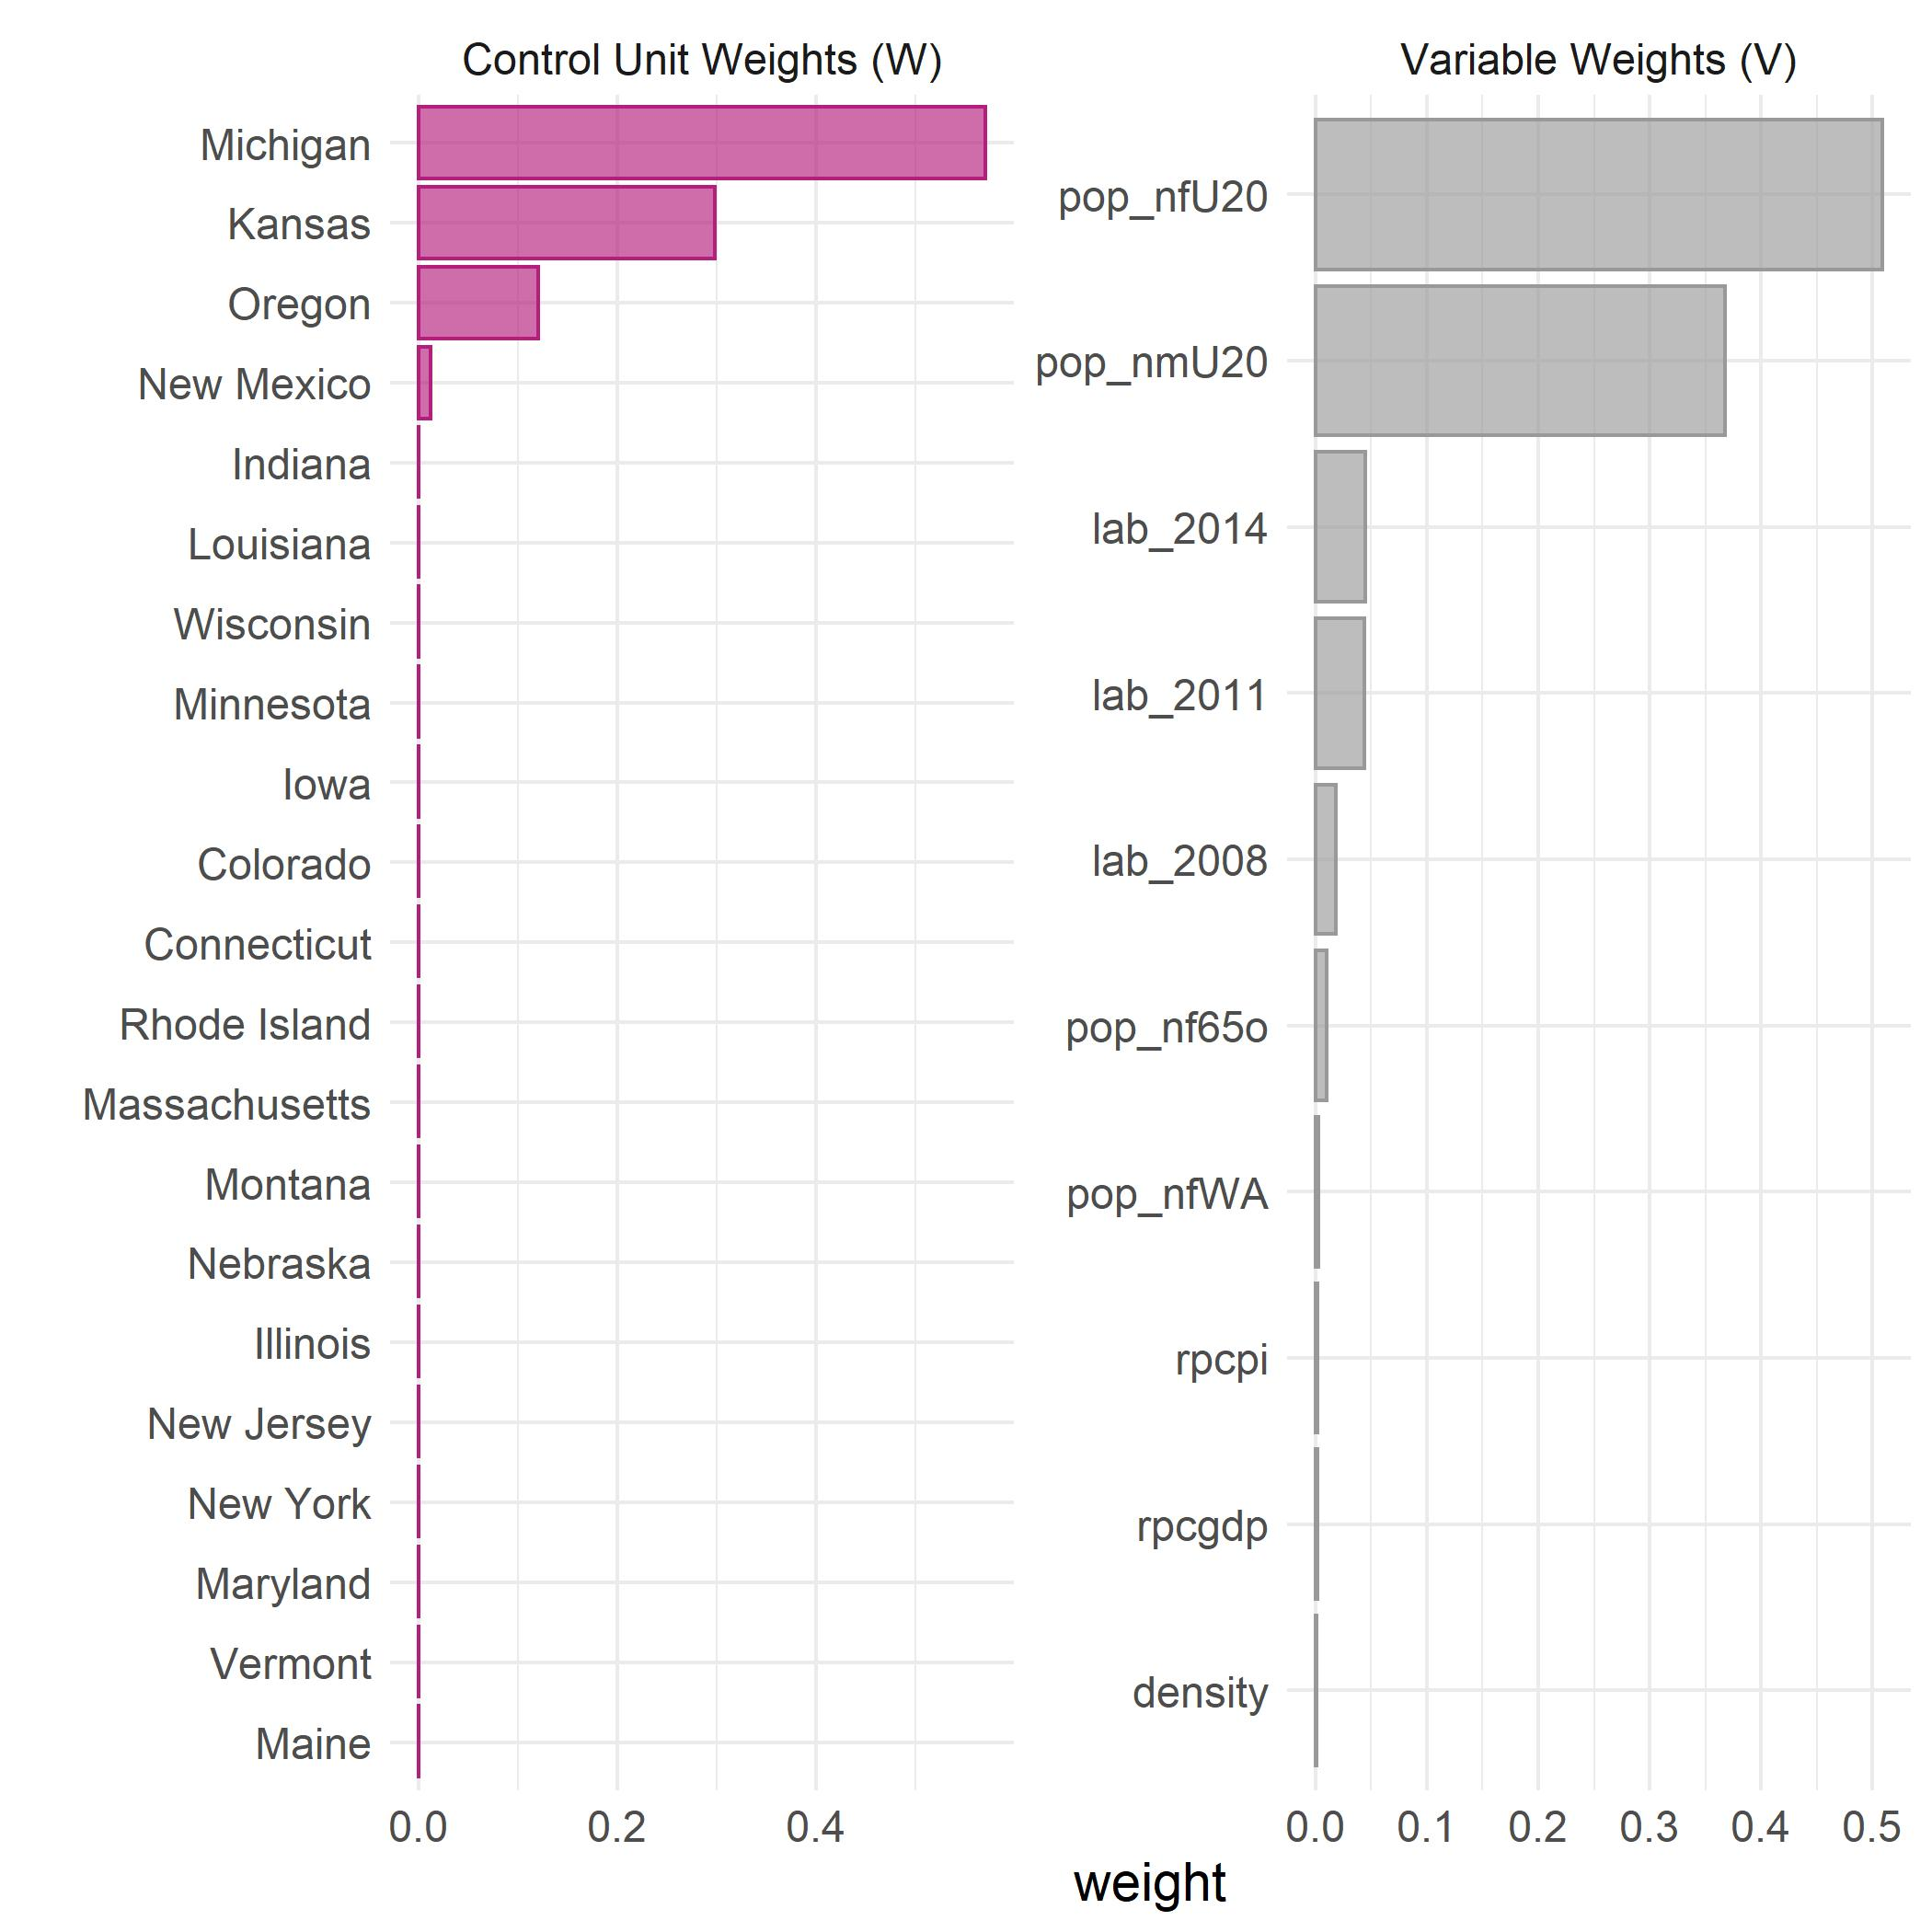
\includegraphics[width=80mm]{nc_lab_weights} &   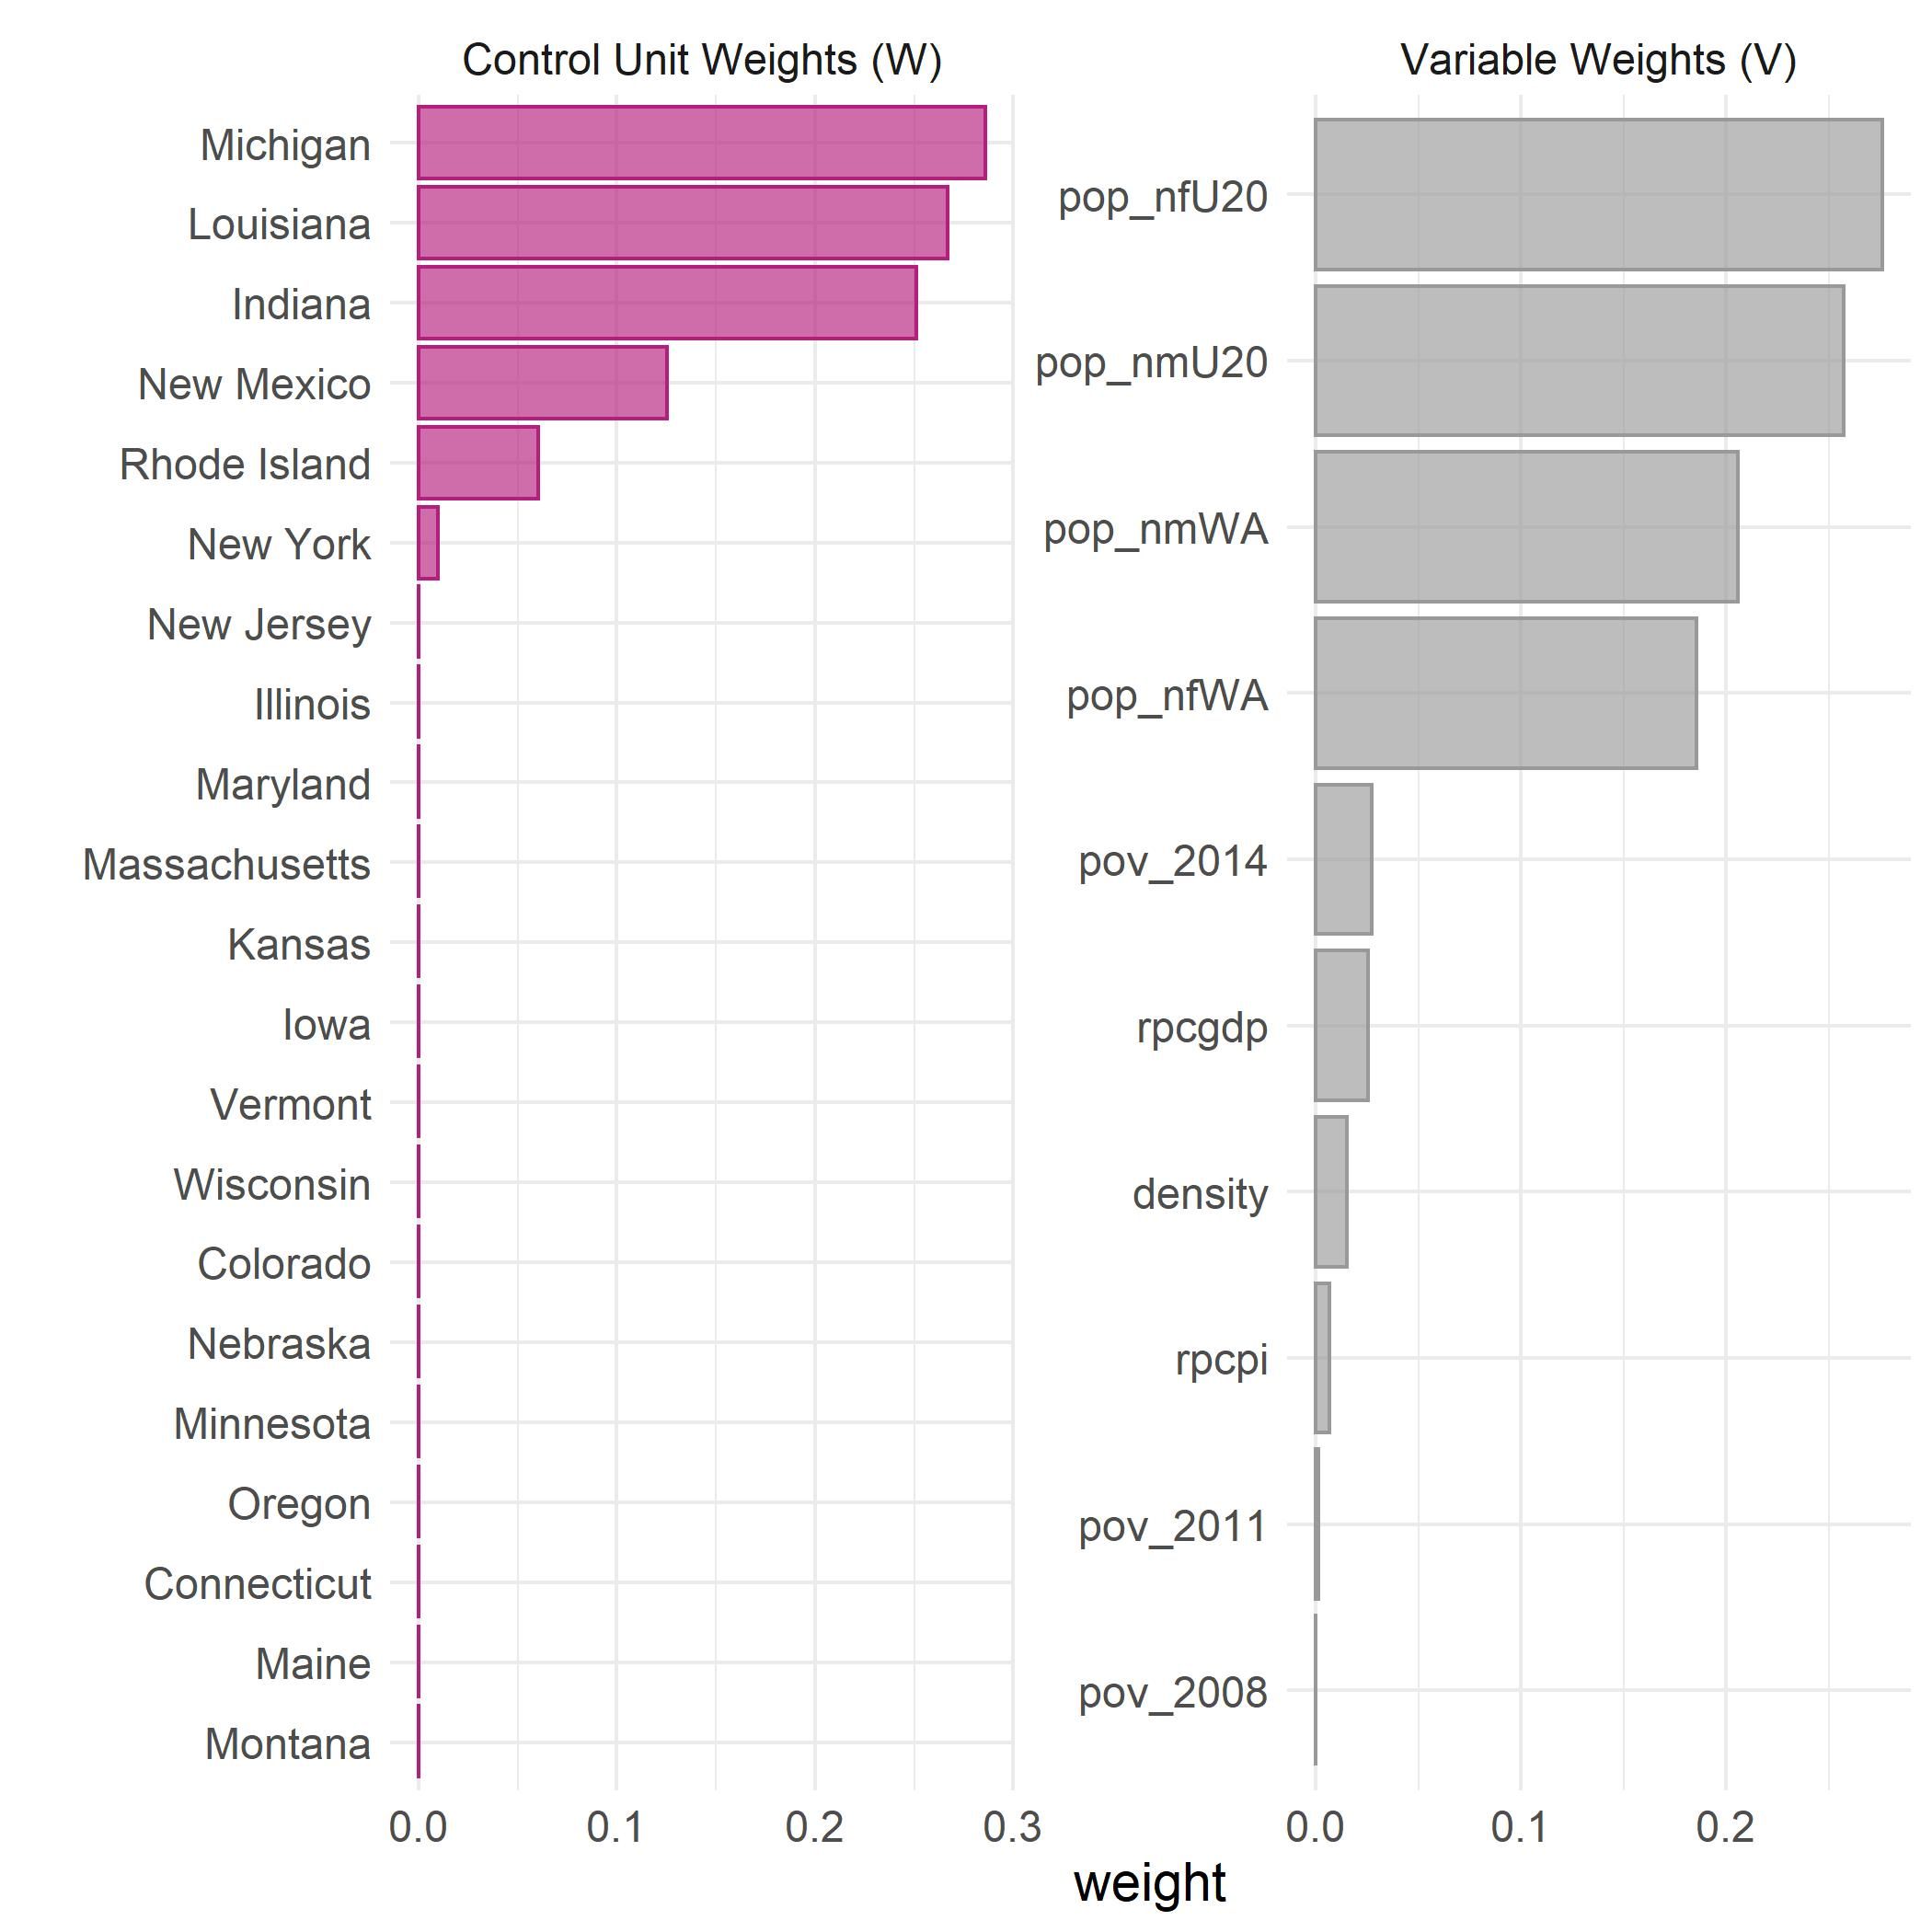
\includegraphics[width=80mm]{nc_pov_weights} \\
\end{tabular}
\end{center}
\label{fig:weights}{}
\end{figure}

\restoregeometry

In order to test the significance of these results, we generate a series of placebos via synthetic control on the states in our control and compare the results as if these states had implemented a similar change in their EITC (either creation or elimination). These allows us to parse the effect from the noise and ask if our results are generated only by chance. This allows to compare the gap of real North Carolina and California with the gaps generated in this process and check if our results are actually meaningful.



 \begin{figure}[H]
    \caption{Poverty Gap in California and Poverty Placebo Gaps}
    \begin{center}
        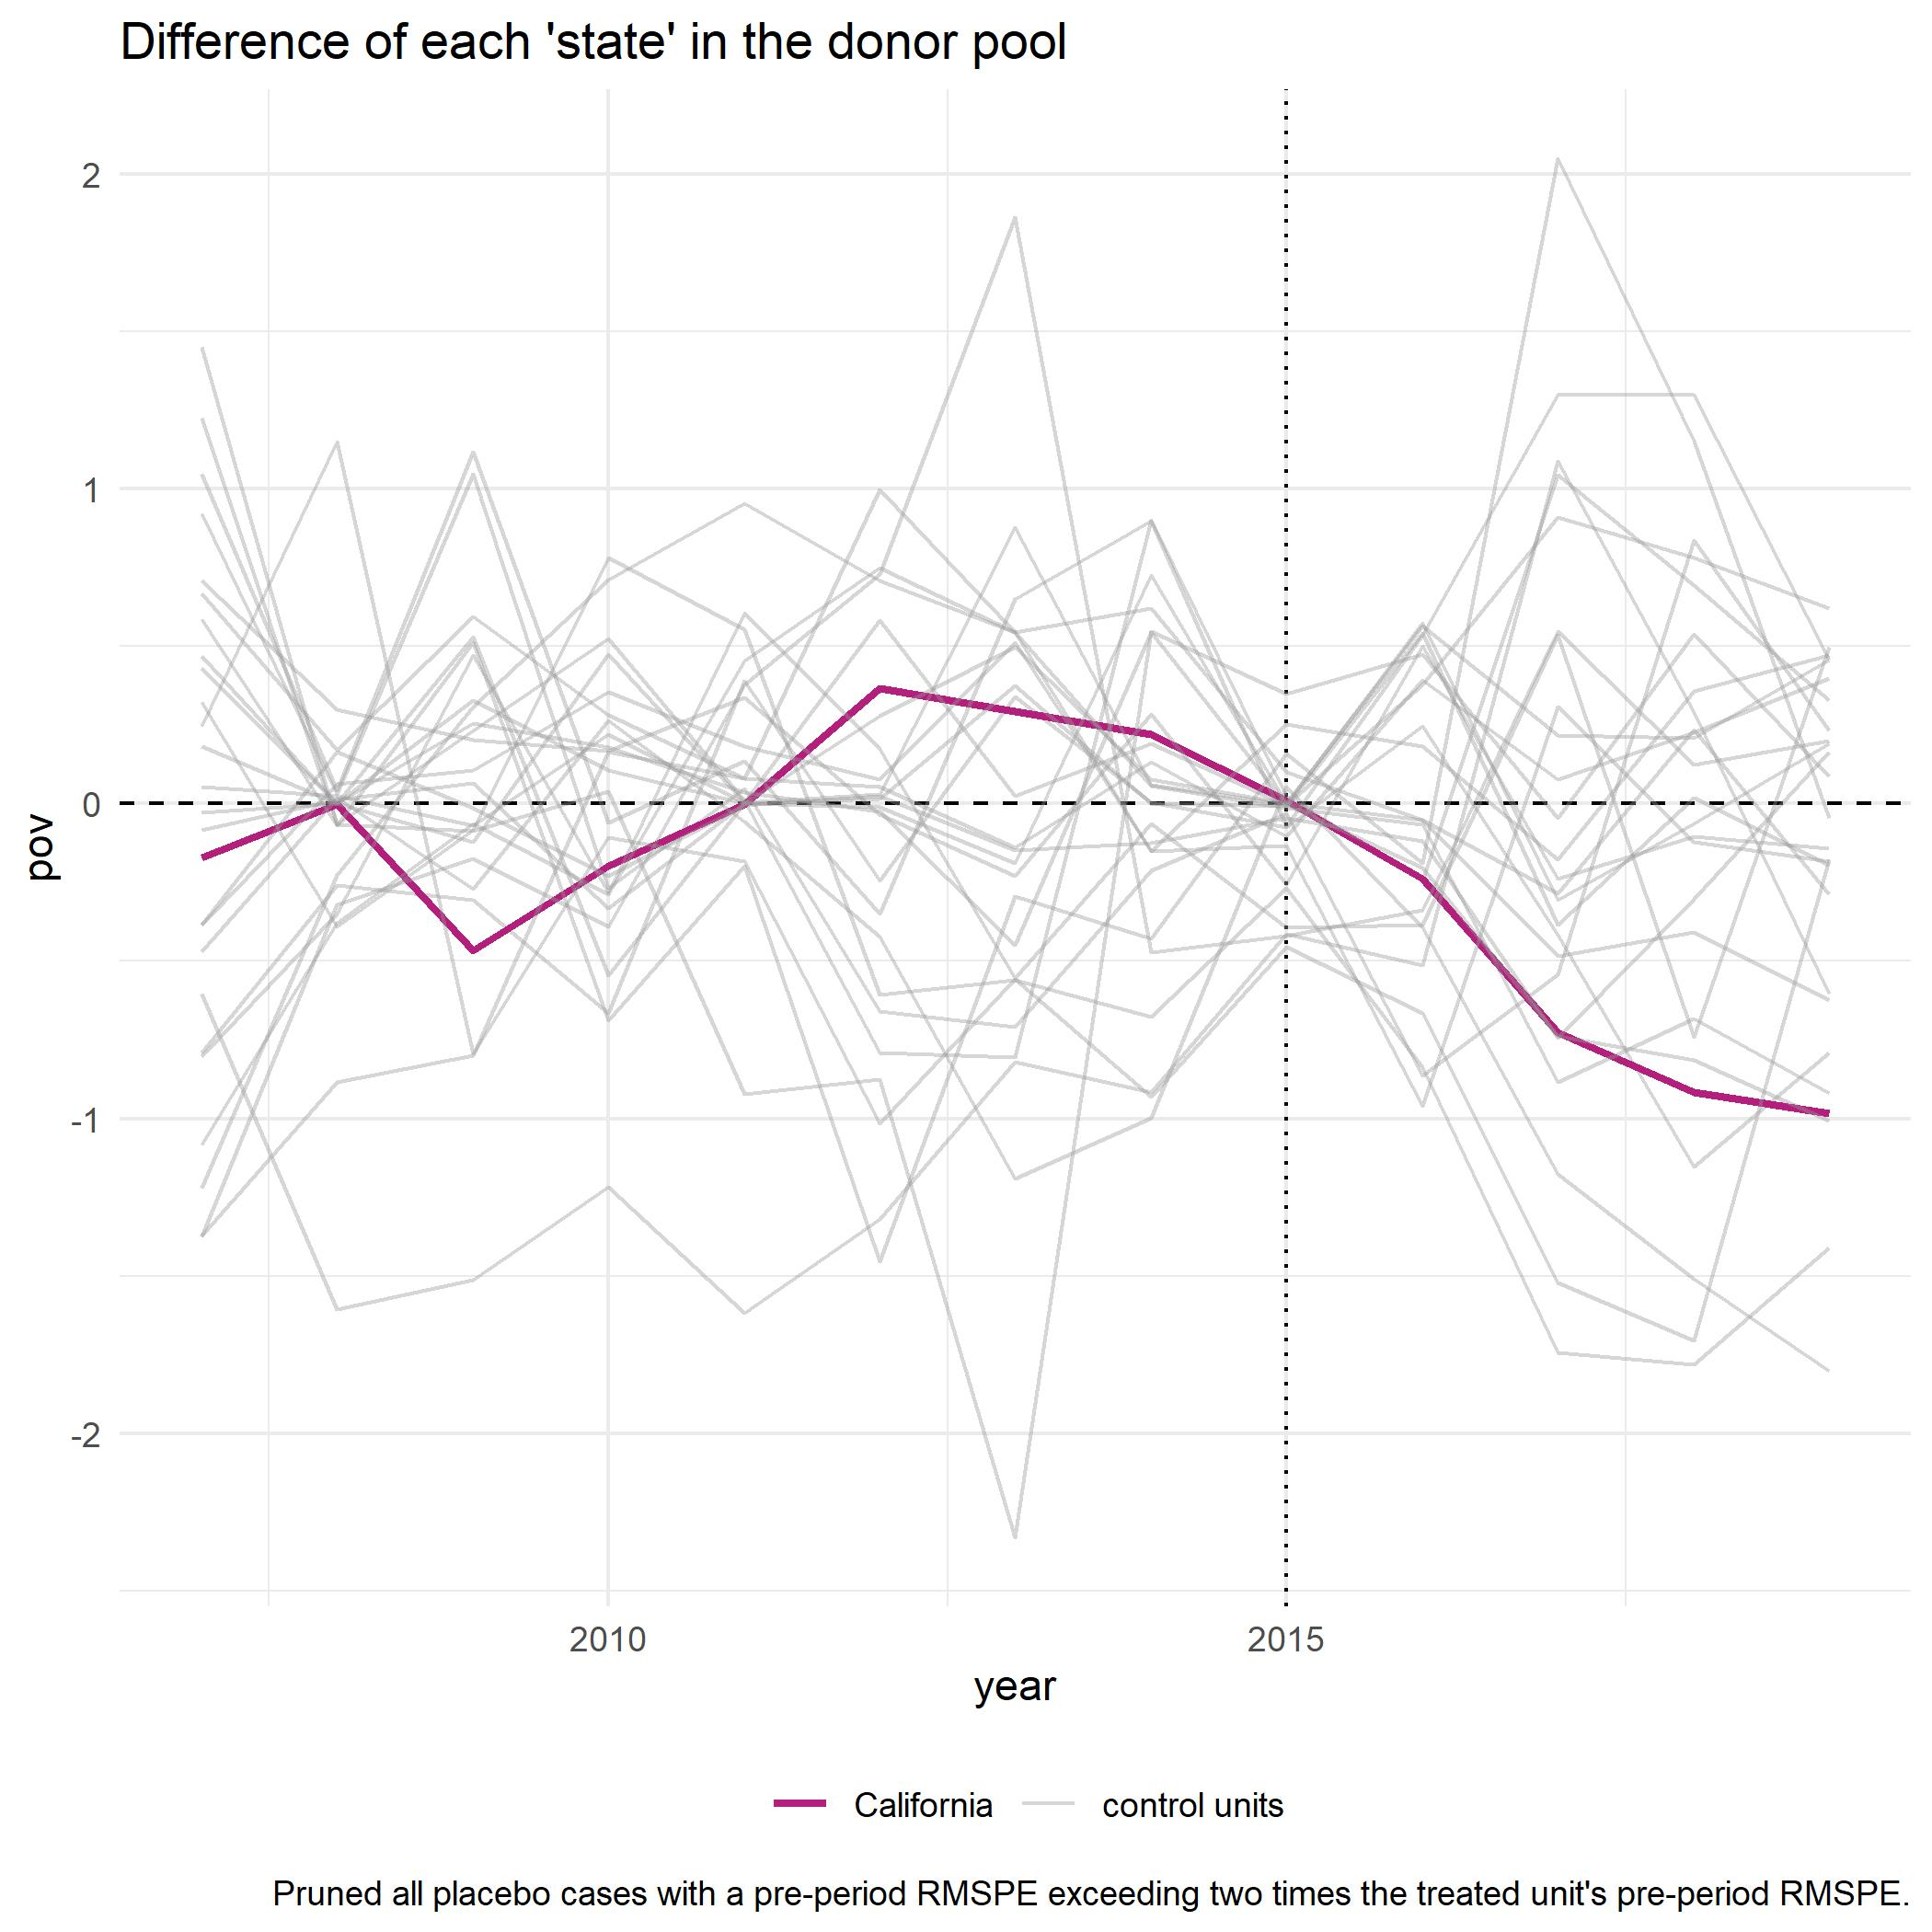
\includegraphics[width=.85\textwidth]{ca_pov_placebos}
    \end{center}
    \label{fig:ca_pov_placebos}{}
\end{figure}

Figure~\ref{fig:ca_pov_placebos} shows a rather inconclusive result. While there is some decrease in poverty following the treatment, there is quite a bit of noise in both the pre-treatment period and in the placebos following treatment. From this, it is difficult to draw any conclusions about CalEITC's impact on the poverty rate in California. A similar result can be seen in Figure~\ref{fig:nc_pov_placebos}, which shows the gap in real North Carolina and the gaps for our synthetic placebos. Once again, there is not a discernably significant impact of the removal of the EITC, even if the directionality of the change in poverty would be the opposite of what economists would predict. 

 \begin{figure}[H]
    \caption{Poverty Gap in North Carolina and Poverty Placebo Gaps}
    \begin{center}
        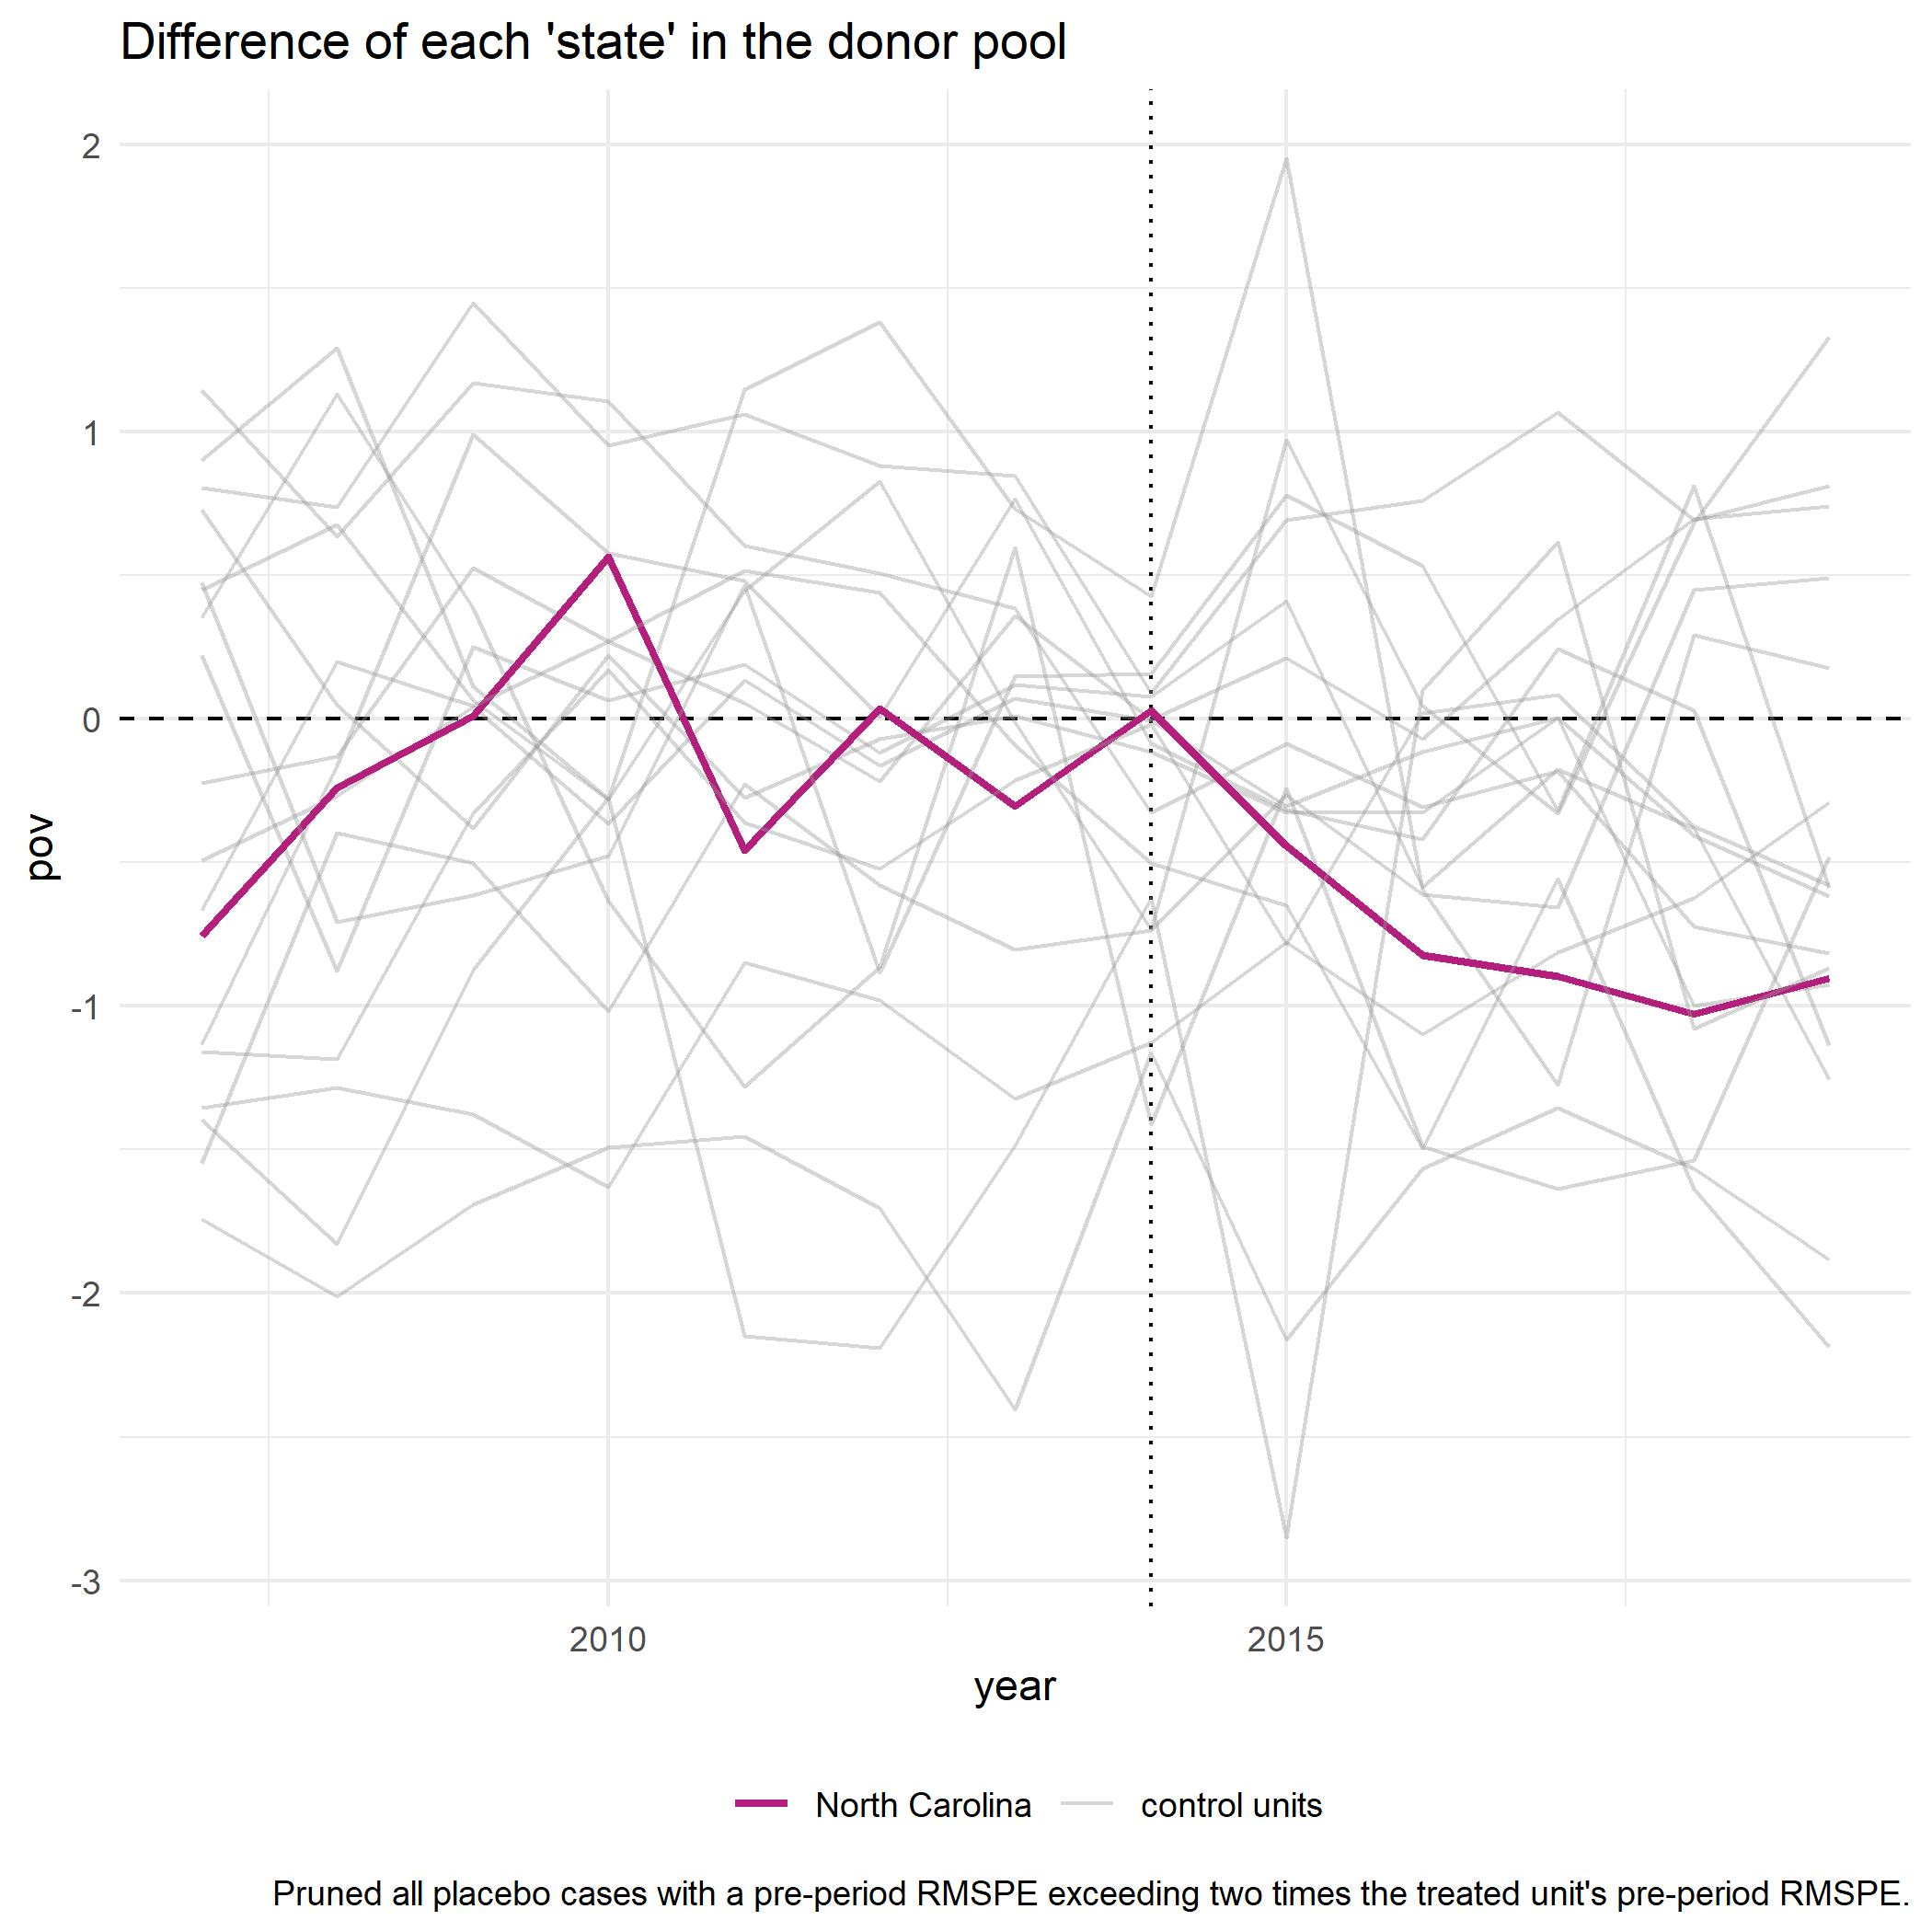
\includegraphics[width=.85\textwidth]{nc_pov_placebos}
    \end{center}
    \label{fig:nc_pov_placebos}{}
\end{figure}

\section{Conclusions}

\bibliography{bib}{}
\bibliographystyle{apalike}

\end{document}
